\documentclass[twoside]{book}

% Packages required by doxygen
\usepackage{fixltx2e}
\usepackage{calc}
\usepackage{doxygen}
\usepackage[export]{adjustbox} % also loads graphicx
\usepackage{graphicx}
\usepackage[utf8]{inputenc}
\usepackage{makeidx}
\usepackage{multicol}
\usepackage{multirow}
\PassOptionsToPackage{warn}{textcomp}
\usepackage{textcomp}
\usepackage[nointegrals]{wasysym}
\usepackage[table]{xcolor}

% Font selection
\usepackage[T1]{fontenc}
\usepackage[scaled=.90]{helvet}
\usepackage{courier}
\usepackage{amssymb}
\usepackage{sectsty}
\renewcommand{\familydefault}{\sfdefault}
\allsectionsfont{%
  \fontseries{bc}\selectfont%
  \color{darkgray}%
}
\renewcommand{\DoxyLabelFont}{%
  \fontseries{bc}\selectfont%
  \color{darkgray}%
}
\newcommand{\+}{\discretionary{\mbox{\scriptsize$\hookleftarrow$}}{}{}}

% Page & text layout
\usepackage{geometry}
\geometry{%
  a4paper,%
  top=2.5cm,%
  bottom=2.5cm,%
  left=2.5cm,%
  right=2.5cm%
}
\tolerance=750
\hfuzz=15pt
\hbadness=750
\setlength{\emergencystretch}{15pt}
\setlength{\parindent}{0cm}
\setlength{\parskip}{3ex plus 2ex minus 2ex}
\makeatletter
\renewcommand{\paragraph}{%
  \@startsection{paragraph}{4}{0ex}{-1.0ex}{1.0ex}{%
    \normalfont\normalsize\bfseries\SS@parafont%
  }%
}
\renewcommand{\subparagraph}{%
  \@startsection{subparagraph}{5}{0ex}{-1.0ex}{1.0ex}{%
    \normalfont\normalsize\bfseries\SS@subparafont%
  }%
}
\makeatother

% Headers & footers
\usepackage{fancyhdr}
\pagestyle{fancyplain}
\fancyhead[LE]{\fancyplain{}{\bfseries\thepage}}
\fancyhead[CE]{\fancyplain{}{}}
\fancyhead[RE]{\fancyplain{}{\bfseries\leftmark}}
\fancyhead[LO]{\fancyplain{}{\bfseries\rightmark}}
\fancyhead[CO]{\fancyplain{}{}}
\fancyhead[RO]{\fancyplain{}{\bfseries\thepage}}
\fancyfoot[LE]{\fancyplain{}{}}
\fancyfoot[CE]{\fancyplain{}{}}
\fancyfoot[RE]{\fancyplain{}{\bfseries\scriptsize Generated by Doxygen }}
\fancyfoot[LO]{\fancyplain{}{\bfseries\scriptsize Generated by Doxygen }}
\fancyfoot[CO]{\fancyplain{}{}}
\fancyfoot[RO]{\fancyplain{}{}}
\renewcommand{\footrulewidth}{0.4pt}
\renewcommand{\chaptermark}[1]{%
  \markboth{#1}{}%
}
\renewcommand{\sectionmark}[1]{%
  \markright{\thesection\ #1}%
}

% Indices & bibliography
\usepackage{natbib}
\usepackage[titles]{tocloft}
\setcounter{tocdepth}{3}
\setcounter{secnumdepth}{5}
\makeindex

% Hyperlinks (required, but should be loaded last)
\usepackage{ifpdf}
\ifpdf
  \usepackage[pdftex,pagebackref=true]{hyperref}
\else
  \usepackage[ps2pdf,pagebackref=true]{hyperref}
\fi
\hypersetup{%
  colorlinks=true,%
  linkcolor=blue,%
  citecolor=blue,%
  unicode%
}

% Custom commands
\newcommand{\clearemptydoublepage}{%
  \newpage{\pagestyle{empty}\cleardoublepage}%
}

\usepackage{caption}
\captionsetup{labelsep=space,justification=centering,font={bf},singlelinecheck=off,skip=4pt,position=top}

%===== C O N T E N T S =====

\begin{document}

% Titlepage & ToC
\hypersetup{pageanchor=false,
             bookmarksnumbered=true,
             pdfencoding=unicode
            }
\pagenumbering{roman}
\begin{titlepage}
\vspace*{7cm}
\begin{center}%
{\Large My Project }\\
\vspace*{1cm}
{\large Generated by Doxygen 1.8.11}\\
\end{center}
\end{titlepage}
\clearemptydoublepage
\tableofcontents
\clearemptydoublepage
\pagenumbering{arabic}
\hypersetup{pageanchor=true}

%--- Begin generated contents ---
\chapter{R\+E\+A\+D\+ME}
\label{md_README}
\hypertarget{md_README}{}
G\+RI Systems

Project consists of following directories, each of which has its’ own Makefile. To run projects’ server , make Makefile in core directory, run the generated executable file using following command\+: ./run.

Next, to run projects’ user, make Makefile in gui directory, run the generated executable file using following command\+: ./gui.

Testing can be accomplished either via G\+UI or terminal.

In terminal type “log login”, after which a login request is sent to server with typed login and default password(ex. log Martijn32). For registration type “reg login”, after which a registration request is sent to server with typed login and default password, name and surname(ex. reg Martijn32). For logging out type “logout”, after which a logout request is sent to server. In order to send messages to another user type “receivers’ login message” (ex. Martijn32 Hello Martijn32, how are you doing?).

First the login window is opened, on users press “\+C\+R\+E\+A\+TE N\+EW A\+C\+C\+O\+U\+N\+T”, after which the registration window is opened, on which users enter their login, password, name and surname to and press “\+Sign\+Up” to complete the registration procedure. On login window users must enter their login and password and press “\+Log\+In” to log in. Finally, after successfully logging in the main window is opened, on which users choose corresponding user from user list, write message in writing area and press “\+Send” button. 
\chapter{Hierarchical Index}
\section{Class Hierarchy}
This inheritance list is sorted roughly, but not completely, alphabetically\+:\begin{DoxyCompactList}
\item \contentsline{section}{Q\+Widget}{\pageref{classQWidget}}{}
\begin{DoxyCompactList}
\item \contentsline{section}{Login\+Window}{\pageref{classLoginWindow}}{}
\item \contentsline{section}{Pop\+Error}{\pageref{classPopError}}{}
\item \contentsline{section}{Registration\+Window}{\pageref{classRegistrationWindow}}{}
\end{DoxyCompactList}
\end{DoxyCompactList}

\chapter{Class Index}
\section{Class List}
Here are the classes, structs, unions and interfaces with brief descriptions\+:\begin{DoxyCompactList}
\item\contentsline{section}{\hyperlink{classLoginWindow}{Login\+Window} \\*Class which creates the G\+UI for login window }{\pageref{classLoginWindow}}{}
\item\contentsline{section}{\hyperlink{classRegistrationWindow}{Registration\+Window} }{\pageref{classRegistrationWindow}}{}
\end{DoxyCompactList}

\chapter{File Index}
\section{File List}
Here is a list of all documented files with brief descriptions\+:\begin{DoxyCompactList}
\item\contentsline{section}{\hyperlink{LoginWindow_8hpp}{Login\+Window.\+hpp} }{\pageref{LoginWindow_8hpp}}{}
\item\contentsline{section}{{\bfseries Registration\+Window.\+hpp} }{\pageref{RegistrationWindow_8hpp}}{}
\end{DoxyCompactList}

\chapter{Class Documentation}
\hypertarget{classAvatar}{}\section{Avatar Class Reference}
\label{classAvatar}\index{Avatar@{Avatar}}


....  




{\ttfamily \#include $<$Avatar.\+hpp$>$}



Inheritance diagram for Avatar\+:
% FIG 0


Collaboration diagram for Avatar\+:
% FIG 1
\subsection*{Public Types}
\begin{DoxyCompactItemize}
\item 
using {\bfseries User} = \hyperlink{classClientUser}{Main\+Window\+::\+User}\hypertarget{classAvatar_a352e86b0217fe9efbfb2fd043d56f74e}{}\label{classAvatar_a352e86b0217fe9efbfb2fd043d56f74e}

\item 
using {\bfseries String} = Main\+Window\+::\+String\hypertarget{classAvatar_a01a9c436ea7bb1e9505aecc22fc10aa0}{}\label{classAvatar_a01a9c436ea7bb1e9505aecc22fc10aa0}

\end{DoxyCompactItemize}
\subsection*{Public Slots}
\begin{DoxyCompactItemize}
\item 
void {\bfseries open\+Conversation} ()\hypertarget{classAvatar_a94dab579111aa83edf4896f0b215be3e}{}\label{classAvatar_a94dab579111aa83edf4896f0b215be3e}

\end{DoxyCompactItemize}
\subsection*{Signals}
\begin{DoxyCompactItemize}
\item 
void {\bfseries clicked} ()\hypertarget{classAvatar_a02690dd056d258245af16d6642cb212b}{}\label{classAvatar_a02690dd056d258245af16d6642cb212b}

\end{DoxyCompactItemize}
\subsection*{Public Member Functions}
\begin{DoxyCompactItemize}
\item 
\hyperlink{classAvatar_a05b18d88147c574d70226e345ba9b681}{Avatar} (\hyperlink{classClientUser}{User} \&, \hyperlink{classMainWindow}{Main\+Window} \&)
\begin{DoxyCompactList}\small\item\em .... \end{DoxyCompactList}\item 
void \hyperlink{classAvatar_a2f3819651922fd0cff31dc504a28e041}{set\+Status} (bool)
\begin{DoxyCompactList}\small\item\em .... \end{DoxyCompactList}\item 
bool \hyperlink{classAvatar_aa764fa2f935fce6b2b4c3c75bc28aba6}{get\+Status} () const 
\begin{DoxyCompactList}\small\item\em .... \end{DoxyCompactList}\item 
void \hyperlink{classAvatar_a316b05699b19fd7f86bd7779d8534feb}{increment\+Count} ()
\begin{DoxyCompactList}\small\item\em .... \end{DoxyCompactList}\item 
const char $\ast$ \hyperlink{classAvatar_ac0739fc3e1ba4ef179389a57d58f078f}{get\+Login} ()
\begin{DoxyCompactList}\small\item\em .... \end{DoxyCompactList}\end{DoxyCompactItemize}


\subsection{Detailed Description}
.... 

\subsection{Constructor \& Destructor Documentation}
\index{Avatar@{Avatar}!Avatar@{Avatar}}
\index{Avatar@{Avatar}!Avatar@{Avatar}}
\subsubsection[{\texorpdfstring{Avatar(\+User \&, Main\+Window \&)}{Avatar(User &, MainWindow &)}}]{\setlength{\rightskip}{0pt plus 5cm}Avatar\+::\+Avatar (
\begin{DoxyParamCaption}
\item[{{\bf User} \&}]{u, }
\item[{{\bf Main\+Window} \&}]{mw}
\end{DoxyParamCaption}
)}\hypertarget{classAvatar_a05b18d88147c574d70226e345ba9b681}{}\label{classAvatar_a05b18d88147c574d70226e345ba9b681}


.... 


\begin{DoxyParams}{Parameters}
{\em ....} & \\
\hline
{\em ....} & \\
\hline
\end{DoxyParams}


\subsection{Member Function Documentation}
\index{Avatar@{Avatar}!get\+Login@{get\+Login}}
\index{get\+Login@{get\+Login}!Avatar@{Avatar}}
\subsubsection[{\texorpdfstring{get\+Login()}{getLogin()}}]{\setlength{\rightskip}{0pt plus 5cm}const char $\ast$ Avatar\+::get\+Login (
\begin{DoxyParamCaption}
{}
\end{DoxyParamCaption}
)}\hypertarget{classAvatar_ac0739fc3e1ba4ef179389a57d58f078f}{}\label{classAvatar_ac0739fc3e1ba4ef179389a57d58f078f}


.... 


\begin{DoxyParams}{Parameters}
{\em no} & parametrs \\
\hline
\end{DoxyParams}
\begin{DoxyReturn}{Returns}
.... 
\end{DoxyReturn}
\index{Avatar@{Avatar}!get\+Status@{get\+Status}}
\index{get\+Status@{get\+Status}!Avatar@{Avatar}}
\subsubsection[{\texorpdfstring{get\+Status() const }{getStatus() const }}]{\setlength{\rightskip}{0pt plus 5cm}bool Avatar\+::get\+Status (
\begin{DoxyParamCaption}
{}
\end{DoxyParamCaption}
) const}\hypertarget{classAvatar_aa764fa2f935fce6b2b4c3c75bc28aba6}{}\label{classAvatar_aa764fa2f935fce6b2b4c3c75bc28aba6}


.... 


\begin{DoxyParams}{Parameters}
{\em no} & parametrs \\
\hline
\end{DoxyParams}
\begin{DoxyReturn}{Returns}
bool 
\end{DoxyReturn}
\index{Avatar@{Avatar}!increment\+Count@{increment\+Count}}
\index{increment\+Count@{increment\+Count}!Avatar@{Avatar}}
\subsubsection[{\texorpdfstring{increment\+Count()}{incrementCount()}}]{\setlength{\rightskip}{0pt plus 5cm}void Avatar\+::increment\+Count (
\begin{DoxyParamCaption}
{}
\end{DoxyParamCaption}
)}\hypertarget{classAvatar_a316b05699b19fd7f86bd7779d8534feb}{}\label{classAvatar_a316b05699b19fd7f86bd7779d8534feb}


.... 


\begin{DoxyParams}{Parameters}
{\em no} & parametrs \\
\hline
\end{DoxyParams}
\begin{DoxyReturn}{Returns}
void 
\end{DoxyReturn}
\index{Avatar@{Avatar}!set\+Status@{set\+Status}}
\index{set\+Status@{set\+Status}!Avatar@{Avatar}}
\subsubsection[{\texorpdfstring{set\+Status(bool)}{setStatus(bool)}}]{\setlength{\rightskip}{0pt plus 5cm}void Avatar\+::set\+Status (
\begin{DoxyParamCaption}
\item[{bool}]{b}
\end{DoxyParamCaption}
)}\hypertarget{classAvatar_a2f3819651922fd0cff31dc504a28e041}{}\label{classAvatar_a2f3819651922fd0cff31dc504a28e041}


.... 


\begin{DoxyParams}{Parameters}
{\em bool} & \\
\hline
\end{DoxyParams}
\begin{DoxyReturn}{Returns}
void 
\end{DoxyReturn}


The documentation for this class was generated from the following files\+:\begin{DoxyCompactItemize}
\item 
gui/\+Main\+Window/\hyperlink{Avatar_8hpp}{Avatar.\+hpp}\item 
gui/\+Main\+Window/Avatar.\+cpp\end{DoxyCompactItemize}

\hypertarget{classClient}{}\section{Client Class Reference}
\label{classClient}\index{Client@{Client}}


Class \hyperlink{classClient}{Client} ....  




{\ttfamily \#include $<$Client.\+hpp$>$}

\subsection*{Public Types}
\begin{DoxyCompactItemize}
\item 
using {\bfseries String} = std\+::string\hypertarget{classClient_a2a46192658d9ba7bb6f9cfa41ce56d11}{}\label{classClient_a2a46192658d9ba7bb6f9cfa41ce56d11}

\end{DoxyCompactItemize}
\subsection*{Public Member Functions}
\begin{DoxyCompactItemize}
\item 
\hyperlink{classClient_ae51af7aa6b8f591496a8f6a4a87a14bf}{Client} ()
\begin{DoxyCompactList}\small\item\em \hyperlink{classClient}{Client} constructor for class \hyperlink{classClient}{Client}. \end{DoxyCompactList}\item 
void \hyperlink{classClient_a1e032189cc8d340550a1a8db868609b2}{connect\+Server} ()
\begin{DoxyCompactList}\small\item\em setup\+And\+Connect calling function create\+Socket, setup\+Address and connect\+Server \end{DoxyCompactList}\item 
void \hyperlink{classClient_a450bc799e79d4a2ef239341b323d38a2}{close\+Connection} ()
\begin{DoxyCompactList}\small\item\em close\+Connection closing socket that comunicated with server? \end{DoxyCompactList}\item 
int \hyperlink{classClient_af4f39b4303028f1e46357f94060ebc2b}{send\+Message} (const String \&)
\begin{DoxyCompactList}\small\item\em send\+Message controling process of sending message if not errors, else asking about errore?? \end{DoxyCompactList}\item 
int \hyperlink{classClient_a81f551d0d21e211e8769adb25a071797}{recv\+Message} (\hyperlink{classTransportLayer}{Transport\+Layer} \&)
\begin{DoxyCompactList}\small\item\em recv\+Message controling process of receiveing message if not errors,else asking about errore?? \end{DoxyCompactList}\end{DoxyCompactItemize}


\subsection{Detailed Description}
Class \hyperlink{classClient}{Client} .... 

\subsection{Constructor \& Destructor Documentation}
\index{Client@{Client}!Client@{Client}}
\index{Client@{Client}!Client@{Client}}
\subsubsection[{\texorpdfstring{Client()}{Client()}}]{\setlength{\rightskip}{0pt plus 5cm}Client\+::\+Client (
\begin{DoxyParamCaption}
{}
\end{DoxyParamCaption}
)}\hypertarget{classClient_ae51af7aa6b8f591496a8f6a4a87a14bf}{}\label{classClient_ae51af7aa6b8f591496a8f6a4a87a14bf}


\hyperlink{classClient}{Client} constructor for class \hyperlink{classClient}{Client}. 


\begin{DoxyParams}{Parameters}
{\em No} & parametrs \\
\hline
\end{DoxyParams}


\subsection{Member Function Documentation}
\index{Client@{Client}!close\+Connection@{close\+Connection}}
\index{close\+Connection@{close\+Connection}!Client@{Client}}
\subsubsection[{\texorpdfstring{close\+Connection()}{closeConnection()}}]{\setlength{\rightskip}{0pt plus 5cm}void Client\+::close\+Connection (
\begin{DoxyParamCaption}
{}
\end{DoxyParamCaption}
)}\hypertarget{classClient_a450bc799e79d4a2ef239341b323d38a2}{}\label{classClient_a450bc799e79d4a2ef239341b323d38a2}


close\+Connection closing socket that comunicated with server? 


\begin{DoxyParams}{Parameters}
{\em no} & parametrs \\
\hline
\end{DoxyParams}
\begin{DoxyReturn}{Returns}
void 
\end{DoxyReturn}
\index{Client@{Client}!connect\+Server@{connect\+Server}}
\index{connect\+Server@{connect\+Server}!Client@{Client}}
\subsubsection[{\texorpdfstring{connect\+Server()}{connectServer()}}]{\setlength{\rightskip}{0pt plus 5cm}void Client\+::connect\+Server (
\begin{DoxyParamCaption}
{}
\end{DoxyParamCaption}
)}\hypertarget{classClient_a1e032189cc8d340550a1a8db868609b2}{}\label{classClient_a1e032189cc8d340550a1a8db868609b2}


setup\+And\+Connect calling function create\+Socket, setup\+Address and connect\+Server 


\begin{DoxyParams}{Parameters}
{\em no} & parametrs \\
\hline
\end{DoxyParams}
\begin{DoxyReturn}{Returns}
void 
\end{DoxyReturn}
\index{Client@{Client}!recv\+Message@{recv\+Message}}
\index{recv\+Message@{recv\+Message}!Client@{Client}}
\subsubsection[{\texorpdfstring{recv\+Message(\+Transport\+Layer \&)}{recvMessage(TransportLayer &)}}]{\setlength{\rightskip}{0pt plus 5cm}int Client\+::recv\+Message (
\begin{DoxyParamCaption}
\item[{{\bf Transport\+Layer} \&}]{tl}
\end{DoxyParamCaption}
)}\hypertarget{classClient_a81f551d0d21e211e8769adb25a071797}{}\label{classClient_a81f551d0d21e211e8769adb25a071797}


recv\+Message controling process of receiveing message if not errors,else asking about errore?? 


\begin{DoxyParams}{Parameters}
{\em Message} & is an initialized string variable \\
\hline
\end{DoxyParams}
\begin{DoxyReturn}{Returns}
Integer 
\end{DoxyReturn}
\index{Client@{Client}!send\+Message@{send\+Message}}
\index{send\+Message@{send\+Message}!Client@{Client}}
\subsubsection[{\texorpdfstring{send\+Message(const String \&)}{sendMessage(const String &)}}]{\setlength{\rightskip}{0pt plus 5cm}int Client\+::send\+Message (
\begin{DoxyParamCaption}
\item[{const String \&}]{message}
\end{DoxyParamCaption}
)}\hypertarget{classClient_af4f39b4303028f1e46357f94060ebc2b}{}\label{classClient_af4f39b4303028f1e46357f94060ebc2b}


send\+Message controling process of sending message if not errors, else asking about errore?? 


\begin{DoxyParams}{Parameters}
{\em Message} & is an initialized string variable \\
\hline
\end{DoxyParams}
\begin{DoxyReturn}{Returns}
Integer 
\end{DoxyReturn}


The documentation for this class was generated from the following files\+:\begin{DoxyCompactItemize}
\item 
core/\hyperlink{Client_8hpp}{Client.\+hpp}\item 
core/Client.\+cpp\end{DoxyCompactItemize}

\hypertarget{classClientUser}{}\section{Client\+User Class Reference}
\label{classClientUser}\index{Client\+User@{Client\+User}}


\hyperlink{classClientUser}{Client\+User} Class.  




{\ttfamily \#include $<$Client\+User.\+hpp$>$}

\subsection*{Public Types}
\begin{DoxyCompactItemize}
\item 
using {\bfseries String} = std\+::string\hypertarget{classClientUser_aef53757bf901527ea25271dcb6bb6f07}{}\label{classClientUser_aef53757bf901527ea25271dcb6bb6f07}

\item 
using {\bfseries Size\+Type} = String\+::size\+\_\+type\hypertarget{classClientUser_a7ae0fc0af4762d5ac0d62b2b74733d63}{}\label{classClientUser_a7ae0fc0af4762d5ac0d62b2b74733d63}

\item 
using {\bfseries Messages} = std\+::list$<$ String $>$\hypertarget{classClientUser_a7edc55abad1cbdfd2eb8ad58ca5a50b1}{}\label{classClientUser_a7edc55abad1cbdfd2eb8ad58ca5a50b1}

\item 
using {\bfseries String\+Ptr} = std\+::shared\+\_\+ptr$<$ String $>$\hypertarget{classClientUser_aa108f0bcb6ad6fa328b18e03e72acef5}{}\label{classClientUser_aa108f0bcb6ad6fa328b18e03e72acef5}

\end{DoxyCompactItemize}
\subsection*{Public Member Functions}
\begin{DoxyCompactItemize}
\item 
\hyperlink{classClientUser_a0c60cdac1feb0952d3b1c1170b1a69bc}{Client\+User} ()\hypertarget{classClientUser_a0c60cdac1feb0952d3b1c1170b1a69bc}{}\label{classClientUser_a0c60cdac1feb0952d3b1c1170b1a69bc}

\begin{DoxyCompactList}\small\item\em \hyperlink{classClientUser}{Client\+User} is constructor for Class \hyperlink{classClientUser}{Client\+User}. \end{DoxyCompactList}\item 
\hyperlink{classClientUser_a0e9c1c34ca28ab22bd0f960ab1ee88f9}{Client\+User} (String \&)
\begin{DoxyCompactList}\small\item\em \hyperlink{classClientUser}{Client\+User} is constructor for Class \hyperlink{classClientUser}{Client\+User}. \end{DoxyCompactList}\item 
bool \hyperlink{classClientUser_aa1fbbd82131fbbab5b468ff12ad7ccaf}{from\+String} (String \&)
\begin{DoxyCompactList}\small\item\em set parametrs login, name, surname, string and check if this empty \end{DoxyCompactList}\item 
void \hyperlink{classClientUser_a34a1353a6b7c4b0c53e621944efc8137}{add\+Message} (const String \&)
\begin{DoxyCompactList}\small\item\em add\+Message asign new message in old mesages and increase by one \end{DoxyCompactList}\item 
String \hyperlink{classClientUser_a73a3633182af0f7ea8cd6534e0d1bbce}{to\+String\+Log} () const 
\begin{DoxyCompactList}\small\item\em to\+String add login name and surname in string \end{DoxyCompactList}\item 
const char $\ast$ \hyperlink{classClientUser_a54826c29f4420a811f65dd7babbf7ad0}{get\+Login} () const 
\begin{DoxyCompactList}\small\item\em get\+Login return login \end{DoxyCompactList}\item 
String \hyperlink{classClientUser_a42db3fc8470f3701f724b47e2d63dc8d}{get\+Name} () const 
\begin{DoxyCompactList}\small\item\em get\+Name return name \end{DoxyCompactList}\item 
String \hyperlink{classClientUser_a9654ca77ca24fa01949feec8d5dc762c}{get\+Surname} () const 
\begin{DoxyCompactList}\small\item\em get\+Surname return surname \end{DoxyCompactList}\item 
bool \hyperlink{classClientUser_ae091b81e5e1ac86a11d3de8135cc36aa}{get\+Status} () const 
\begin{DoxyCompactList}\small\item\em get\+Status return status \end{DoxyCompactList}\item 
Size\+Type \hyperlink{classClientUser_aad8dc8d49e94f68a8bbbe324a55e68d9}{get\+Unread\+Messages\+Count} () const 
\begin{DoxyCompactList}\small\item\em get\+Unread\+Messages\+Count return unread messages count \end{DoxyCompactList}\item 
Messages \& \hyperlink{classClientUser_a1cb9cc387ca7e6fb374f9745409ad552}{get\+Messages} ()
\begin{DoxyCompactList}\small\item\em get\+Messages return messages \end{DoxyCompactList}\item 
void \hyperlink{classClientUser_a9fc92b13a43c208773ea25aade33ba54}{set\+Status} (const bool)
\begin{DoxyCompactList}\small\item\em asigne the value to status \end{DoxyCompactList}\item 
void \hyperlink{classClientUser_afa0747fa782b945e0f1430605dde5f4e}{set\+Unread\+Messages} (const Size\+Type)
\begin{DoxyCompactList}\small\item\em asign the value to unread messages \end{DoxyCompactList}\item 
\hyperlink{classClientUser}{Client\+User} $\ast$ \hyperlink{classClientUser_a8144e58927e95bff49485c3a81c40893}{get\+Pointer} ()
\begin{DoxyCompactList}\small\item\em ... \end{DoxyCompactList}\end{DoxyCompactItemize}


\subsection{Detailed Description}
\hyperlink{classClientUser}{Client\+User} Class. 

\subsection{Constructor \& Destructor Documentation}
\index{Client\+User@{Client\+User}!Client\+User@{Client\+User}}
\index{Client\+User@{Client\+User}!Client\+User@{Client\+User}}
\subsubsection[{\texorpdfstring{Client\+User(\+String \&)}{ClientUser(String &)}}]{\setlength{\rightskip}{0pt plus 5cm}Client\+User\+::\+Client\+User (
\begin{DoxyParamCaption}
\item[{String \&}]{client\+Str}
\end{DoxyParamCaption}
)\hspace{0.3cm}{\ttfamily [explicit]}}\hypertarget{classClientUser_a0e9c1c34ca28ab22bd0f960ab1ee88f9}{}\label{classClientUser_a0e9c1c34ca28ab22bd0f960ab1ee88f9}


\hyperlink{classClientUser}{Client\+User} is constructor for Class \hyperlink{classClientUser}{Client\+User}. 


\begin{DoxyParams}{Parameters}
{\em Reference} & of String \\
\hline
\end{DoxyParams}


\subsection{Member Function Documentation}
\index{Client\+User@{Client\+User}!add\+Message@{add\+Message}}
\index{add\+Message@{add\+Message}!Client\+User@{Client\+User}}
\subsubsection[{\texorpdfstring{add\+Message(const String \&)}{addMessage(const String &)}}]{\setlength{\rightskip}{0pt plus 5cm}void Client\+User\+::add\+Message (
\begin{DoxyParamCaption}
\item[{const String \&}]{message}
\end{DoxyParamCaption}
)}\hypertarget{classClientUser_a34a1353a6b7c4b0c53e621944efc8137}{}\label{classClientUser_a34a1353a6b7c4b0c53e621944efc8137}


add\+Message asign new message in old mesages and increase by one 


\begin{DoxyParams}{Parameters}
{\em const} & reference of String?? \\
\hline
\end{DoxyParams}
\begin{DoxyReturn}{Returns}
void 
\end{DoxyReturn}
\index{Client\+User@{Client\+User}!from\+String@{from\+String}}
\index{from\+String@{from\+String}!Client\+User@{Client\+User}}
\subsubsection[{\texorpdfstring{from\+String(\+String \&)}{fromString(String &)}}]{\setlength{\rightskip}{0pt plus 5cm}bool Client\+User\+::from\+String (
\begin{DoxyParamCaption}
\item[{String \&}]{client\+Str}
\end{DoxyParamCaption}
)}\hypertarget{classClientUser_aa1fbbd82131fbbab5b468ff12ad7ccaf}{}\label{classClientUser_aa1fbbd82131fbbab5b468ff12ad7ccaf}


set parametrs login, name, surname, string and check if this empty 


\begin{DoxyParams}{Parameters}
{\em Reference} & of String \\
\hline
\end{DoxyParams}
\begin{DoxyReturn}{Returns}
bool parametr 
\end{DoxyReturn}
\index{Client\+User@{Client\+User}!get\+Login@{get\+Login}}
\index{get\+Login@{get\+Login}!Client\+User@{Client\+User}}
\subsubsection[{\texorpdfstring{get\+Login() const }{getLogin() const }}]{\setlength{\rightskip}{0pt plus 5cm}const char $\ast$ Client\+User\+::get\+Login (
\begin{DoxyParamCaption}
{}
\end{DoxyParamCaption}
) const}\hypertarget{classClientUser_a54826c29f4420a811f65dd7babbf7ad0}{}\label{classClientUser_a54826c29f4420a811f65dd7babbf7ad0}


get\+Login return login 


\begin{DoxyParams}{Parameters}
{\em no} & parametrs \\
\hline
\end{DoxyParams}
\begin{DoxyReturn}{Returns}
String 
\end{DoxyReturn}
\index{Client\+User@{Client\+User}!get\+Messages@{get\+Messages}}
\index{get\+Messages@{get\+Messages}!Client\+User@{Client\+User}}
\subsubsection[{\texorpdfstring{get\+Messages()}{getMessages()}}]{\setlength{\rightskip}{0pt plus 5cm}Client\+User\+::\+Messages \& Client\+User\+::get\+Messages (
\begin{DoxyParamCaption}
{}
\end{DoxyParamCaption}
)}\hypertarget{classClientUser_a1cb9cc387ca7e6fb374f9745409ad552}{}\label{classClientUser_a1cb9cc387ca7e6fb374f9745409ad552}


get\+Messages return messages 


\begin{DoxyParams}{Parameters}
{\em no} & parametrs \\
\hline
\end{DoxyParams}
\begin{DoxyReturn}{Returns}
???... 
\end{DoxyReturn}
\index{Client\+User@{Client\+User}!get\+Name@{get\+Name}}
\index{get\+Name@{get\+Name}!Client\+User@{Client\+User}}
\subsubsection[{\texorpdfstring{get\+Name() const }{getName() const }}]{\setlength{\rightskip}{0pt plus 5cm}String Client\+User\+::get\+Name (
\begin{DoxyParamCaption}
{}
\end{DoxyParamCaption}
) const}\hypertarget{classClientUser_a42db3fc8470f3701f724b47e2d63dc8d}{}\label{classClientUser_a42db3fc8470f3701f724b47e2d63dc8d}


get\+Name return name 


\begin{DoxyParams}{Parameters}
{\em no} & parametrs \\
\hline
\end{DoxyParams}
\begin{DoxyReturn}{Returns}
String 
\end{DoxyReturn}
\index{Client\+User@{Client\+User}!get\+Pointer@{get\+Pointer}}
\index{get\+Pointer@{get\+Pointer}!Client\+User@{Client\+User}}
\subsubsection[{\texorpdfstring{get\+Pointer()}{getPointer()}}]{\setlength{\rightskip}{0pt plus 5cm}{\bf Client\+User} $\ast$ Client\+User\+::get\+Pointer (
\begin{DoxyParamCaption}
{}
\end{DoxyParamCaption}
)}\hypertarget{classClientUser_a8144e58927e95bff49485c3a81c40893}{}\label{classClientUser_a8144e58927e95bff49485c3a81c40893}


... 


\begin{DoxyParams}{Parameters}
{\em no} & parametrs \\
\hline
\end{DoxyParams}
\begin{DoxyReturn}{Returns}
... 
\end{DoxyReturn}
\index{Client\+User@{Client\+User}!get\+Status@{get\+Status}}
\index{get\+Status@{get\+Status}!Client\+User@{Client\+User}}
\subsubsection[{\texorpdfstring{get\+Status() const }{getStatus() const }}]{\setlength{\rightskip}{0pt plus 5cm}bool Client\+User\+::get\+Status (
\begin{DoxyParamCaption}
{}
\end{DoxyParamCaption}
) const}\hypertarget{classClientUser_ae091b81e5e1ac86a11d3de8135cc36aa}{}\label{classClientUser_ae091b81e5e1ac86a11d3de8135cc36aa}


get\+Status return status 


\begin{DoxyParams}{Parameters}
{\em no} & parametrs \\
\hline
\end{DoxyParams}
\begin{DoxyReturn}{Returns}
bool 
\end{DoxyReturn}
\index{Client\+User@{Client\+User}!get\+Surname@{get\+Surname}}
\index{get\+Surname@{get\+Surname}!Client\+User@{Client\+User}}
\subsubsection[{\texorpdfstring{get\+Surname() const }{getSurname() const }}]{\setlength{\rightskip}{0pt plus 5cm}String Client\+User\+::get\+Surname (
\begin{DoxyParamCaption}
{}
\end{DoxyParamCaption}
) const}\hypertarget{classClientUser_a9654ca77ca24fa01949feec8d5dc762c}{}\label{classClientUser_a9654ca77ca24fa01949feec8d5dc762c}


get\+Surname return surname 


\begin{DoxyParams}{Parameters}
{\em no} & parametrs \\
\hline
\end{DoxyParams}
\begin{DoxyReturn}{Returns}
String 
\end{DoxyReturn}
\index{Client\+User@{Client\+User}!get\+Unread\+Messages\+Count@{get\+Unread\+Messages\+Count}}
\index{get\+Unread\+Messages\+Count@{get\+Unread\+Messages\+Count}!Client\+User@{Client\+User}}
\subsubsection[{\texorpdfstring{get\+Unread\+Messages\+Count() const }{getUnreadMessagesCount() const }}]{\setlength{\rightskip}{0pt plus 5cm}Client\+User\+::\+Size\+Type Client\+User\+::get\+Unread\+Messages\+Count (
\begin{DoxyParamCaption}
{}
\end{DoxyParamCaption}
) const}\hypertarget{classClientUser_aad8dc8d49e94f68a8bbbe324a55e68d9}{}\label{classClientUser_aad8dc8d49e94f68a8bbbe324a55e68d9}


get\+Unread\+Messages\+Count return unread messages count 


\begin{DoxyParams}{Parameters}
{\em no} & parametrs \\
\hline
\end{DoxyParams}
\begin{DoxyReturn}{Returns}
Size\+Type,it\textquotesingle{}s size of string 
\end{DoxyReturn}
\index{Client\+User@{Client\+User}!set\+Status@{set\+Status}}
\index{set\+Status@{set\+Status}!Client\+User@{Client\+User}}
\subsubsection[{\texorpdfstring{set\+Status(const bool)}{setStatus(const bool)}}]{\setlength{\rightskip}{0pt plus 5cm}void Client\+User\+::set\+Status (
\begin{DoxyParamCaption}
\item[{const bool}]{st}
\end{DoxyParamCaption}
)}\hypertarget{classClientUser_a9fc92b13a43c208773ea25aade33ba54}{}\label{classClientUser_a9fc92b13a43c208773ea25aade33ba54}


asigne the value to status 


\begin{DoxyParams}{Parameters}
{\em const} & bool parametr? \\
\hline
\end{DoxyParams}
\begin{DoxyReturn}{Returns}
void 
\end{DoxyReturn}
\index{Client\+User@{Client\+User}!set\+Unread\+Messages@{set\+Unread\+Messages}}
\index{set\+Unread\+Messages@{set\+Unread\+Messages}!Client\+User@{Client\+User}}
\subsubsection[{\texorpdfstring{set\+Unread\+Messages(const Size\+Type)}{setUnreadMessages(const SizeType)}}]{\setlength{\rightskip}{0pt plus 5cm}void Client\+User\+::set\+Unread\+Messages (
\begin{DoxyParamCaption}
\item[{const Size\+Type}]{um}
\end{DoxyParamCaption}
)}\hypertarget{classClientUser_afa0747fa782b945e0f1430605dde5f4e}{}\label{classClientUser_afa0747fa782b945e0f1430605dde5f4e}


asign the value to unread messages 


\begin{DoxyParams}{Parameters}
{\em size} & of string \\
\hline
\end{DoxyParams}
\begin{DoxyReturn}{Returns}
void 
\end{DoxyReturn}
\index{Client\+User@{Client\+User}!to\+String\+Log@{to\+String\+Log}}
\index{to\+String\+Log@{to\+String\+Log}!Client\+User@{Client\+User}}
\subsubsection[{\texorpdfstring{to\+String\+Log() const }{toStringLog() const }}]{\setlength{\rightskip}{0pt plus 5cm}String Client\+User\+::to\+String\+Log (
\begin{DoxyParamCaption}
{}
\end{DoxyParamCaption}
) const}\hypertarget{classClientUser_a73a3633182af0f7ea8cd6534e0d1bbce}{}\label{classClientUser_a73a3633182af0f7ea8cd6534e0d1bbce}


to\+String add login name and surname in string 


\begin{DoxyParams}{Parameters}
{\em no} & parametrs \\
\hline
\end{DoxyParams}
\begin{DoxyReturn}{Returns}
String 
\end{DoxyReturn}


The documentation for this class was generated from the following files\+:\begin{DoxyCompactItemize}
\item 
core/\hyperlink{ClientUser_8hpp}{Client\+User.\+hpp}\item 
core/Client\+User.\+cpp\end{DoxyCompactItemize}

\hypertarget{classController}{}\section{Controller Class Reference}
\label{classController}\index{Controller@{Controller}}
\subsection*{Classes}
\begin{DoxyCompactItemize}
\item 
class \hyperlink{classController_1_1InputReader}{Input\+Reader}
\end{DoxyCompactItemize}
\subsection*{Public Types}
\begin{DoxyCompactItemize}
\item 
using {\bfseries User} = \hyperlink{classClientUser}{Client\+User}\hypertarget{classController_ae8e4814b1b057df2b338500d286a6dd3}{}\label{classController_ae8e4814b1b057df2b338500d286a6dd3}

\item 
using {\bfseries Users} = std\+::list$<$ \hyperlink{classClientUser}{User} $>$\hypertarget{classController_ac0c64a258282568b1fe458447b58cdec}{}\label{classController_ac0c64a258282568b1fe458447b58cdec}

\item 
using {\bfseries User\+Iter} = Users\+::iterator\hypertarget{classController_ac9e8c85fbff11efe305273c65e51cb0f}{}\label{classController_ac9e8c85fbff11efe305273c65e51cb0f}

\item 
using {\bfseries String} = User\+::\+String\hypertarget{classController_a544a3f0a0e5bfb251cfdd457b62374f0}{}\label{classController_a544a3f0a0e5bfb251cfdd457b62374f0}

\end{DoxyCompactItemize}
\subsection*{Public Member Functions}
\begin{DoxyCompactItemize}
\item 
{\bfseries Controller} (\hyperlink{classClient}{Client} \&)\hypertarget{classController_abdfa33e6687675dbcece03f3b71f7ad0}{}\label{classController_abdfa33e6687675dbcece03f3b71f7ad0}

\item 
void {\bfseries run} (const String \&)\hypertarget{classController_a8dc70c84e6d5c77b6801073f17a09c9f}{}\label{classController_a8dc70c84e6d5c77b6801073f17a09c9f}

\item 
void {\bfseries handle\+Session} ()\hypertarget{classController_a55b91f599170dc6e7b0dc01c6560c474}{}\label{classController_a55b91f599170dc6e7b0dc01c6560c474}

\item 
String {\bfseries send\+Login\+Request} (const String \&login, const String \&password)\hypertarget{classController_a554f7fefaf160170986f4b916aeb4ffd}{}\label{classController_a554f7fefaf160170986f4b916aeb4ffd}

\item 
String {\bfseries send\+Logout\+Request} ()\hypertarget{classController_a6919677cbe8e89171c99544860c07ce6}{}\label{classController_a6919677cbe8e89171c99544860c07ce6}

\item 
String {\bfseries send\+Registration\+Request} (const String \&login, const String \&name, const String \&surname, const String \&password)\hypertarget{classController_a1b3e4b042a20b1f94010eb6625e3ac20}{}\label{classController_a1b3e4b042a20b1f94010eb6625e3ac20}

\item 
String {\bfseries send\+Message\+To\+User} (const String \&to\+User, String \&msg)\hypertarget{classController_a3663c7529e007675c1e94ead6d5aafc9}{}\label{classController_a3663c7529e007675c1e94ead6d5aafc9}

\item 
String {\bfseries send\+Conv\+Request} (const String \&)\hypertarget{classController_a774bfb89454e8ae116c1ba51395d6392}{}\label{classController_a774bfb89454e8ae116c1ba51395d6392}

\item 
void {\bfseries f} (String \&str)\hypertarget{classController_a95e98a70661457e6d3d08a0985ebe72d}{}\label{classController_a95e98a70661457e6d3d08a0985ebe72d}

\item 
String {\bfseries get\+Login} () const \hypertarget{classController_aad5de5df0deb5c552c0b6c57acabee26}{}\label{classController_aad5de5df0deb5c552c0b6c57acabee26}

\end{DoxyCompactItemize}


The documentation for this class was generated from the following files\+:\begin{DoxyCompactItemize}
\item 
core/\hyperlink{Controller_8hpp}{Controller.\+hpp}\item 
core/Controller.\+cpp\end{DoxyCompactItemize}

\hypertarget{classConversation}{}\section{Conversation Class Reference}
\label{classConversation}\index{Conversation@{Conversation}}
\subsection*{Public Types}
\begin{DoxyCompactItemize}
\item 
using {\bfseries String} = std\+::string\hypertarget{classConversation_a2b431b2bafb50e15aec52141053a5d2b}{}\label{classConversation_a2b431b2bafb50e15aec52141053a5d2b}

\item 
using {\bfseries Size\+Type} = String\+::size\+\_\+type\hypertarget{classConversation_a736667fdf70fd1ed56e990a53ffb2e5e}{}\label{classConversation_a736667fdf70fd1ed56e990a53ffb2e5e}

\item 
using {\bfseries Conv} = std\+::list$<$ String $>$\hypertarget{classConversation_ad0d8c118486f9b7bbd1099ededd6ea7f}{}\label{classConversation_ad0d8c118486f9b7bbd1099ededd6ea7f}

\item 
using {\bfseries Conv\+Ptr} = std\+::shared\+\_\+ptr$<$ Conv $>$\hypertarget{classConversation_a3fc3feaa732bef68eb5f504ae3b79a62}{}\label{classConversation_a3fc3feaa732bef68eb5f504ae3b79a62}

\end{DoxyCompactItemize}
\subsection*{Public Member Functions}
\begin{DoxyCompactItemize}
\item 
{\bfseries Conversation} (const String \&, const String \&)\hypertarget{classConversation_ad464ef676935998f598ac83d6dfc5259}{}\label{classConversation_ad464ef676935998f598ac83d6dfc5259}

\item 
bool {\bfseries equal} (const String \&u1, const String \&u2) const \hypertarget{classConversation_a729fc80b6ac75c1cac223a3d1a3c4743}{}\label{classConversation_a729fc80b6ac75c1cac223a3d1a3c4743}

\item 
void {\bfseries add\+Message} (const String \&msg)\hypertarget{classConversation_a5fc239d548391b6c582ac9b2d8c2893b}{}\label{classConversation_a5fc239d548391b6c582ac9b2d8c2893b}

\item 
Conv\+Ptr {\bfseries get\+Conversation} ()\hypertarget{classConversation_ac85deef748d90bb03b01ce9fcc27fced}{}\label{classConversation_ac85deef748d90bb03b01ce9fcc27fced}

\end{DoxyCompactItemize}


The documentation for this class was generated from the following files\+:\begin{DoxyCompactItemize}
\item 
core/Conversation.\+hpp\item 
core/Conversation.\+cpp\end{DoxyCompactItemize}

\hypertarget{classDBController}{}\section{D\+B\+Controller$<$ Users $>$ Class Template Reference}
\label{classDBController}\index{D\+B\+Controller$<$ Users $>$@{D\+B\+Controller$<$ Users $>$}}
\subsection*{Public Types}
\begin{DoxyCompactItemize}
\item 
using {\bfseries User} = typename Users\+::value\+\_\+type\hypertarget{classDBController_ab621e56636010ffa790768031b6e1f58}{}\label{classDBController_ab621e56636010ffa790768031b6e1f58}

\item 
using {\bfseries String} = std\+::string\hypertarget{classDBController_afc05cf46913445cad521510401ba915c}{}\label{classDBController_afc05cf46913445cad521510401ba915c}

\item 
using {\bfseries mut\+Guard} = std\+::lock\+\_\+guard$<$ std\+::mutex $>$\hypertarget{classDBController_a2cc84030c82e94f79cd6f0da5a49a4ee}{}\label{classDBController_a2cc84030c82e94f79cd6f0da5a49a4ee}

\item 
using {\bfseries Conversations} = std\+::list$<$ \hyperlink{classConversation}{Conversation} $>$\hypertarget{classDBController_a72de5ce4988f74484b295dd24b699f55}{}\label{classDBController_a72de5ce4988f74484b295dd24b699f55}

\item 
using {\bfseries Conv\+Iter} = Conversations\+::iterator\hypertarget{classDBController_aede4241d22b2ab7a23a9311efc45b9c3}{}\label{classDBController_aede4241d22b2ab7a23a9311efc45b9c3}

\item 
using {\bfseries Conv\+Ptr} = Conversation\+::\+Conv\+Ptr\hypertarget{classDBController_ab3f8ef368bebfd895073943f20b4b302}{}\label{classDBController_ab3f8ef368bebfd895073943f20b4b302}

\item 
using {\bfseries P\+Messages} = Server\+User\+::\+Pending\+Messages\hypertarget{classDBController_a54f4ce4e32b7f1e2cfe5f0108e4e118b}{}\label{classDBController_a54f4ce4e32b7f1e2cfe5f0108e4e118b}

\item 
using {\bfseries P\+Messages\+Ptr} = Server\+User\+::\+P\+Messages\+Ptr\hypertarget{classDBController_ae2dd2067bcc0998090de4ddc1edd6be2}{}\label{classDBController_ae2dd2067bcc0998090de4ddc1edd6be2}

\end{DoxyCompactItemize}
\subsection*{Public Member Functions}
\begin{DoxyCompactItemize}
\item 
{\bfseries D\+B\+Controller} (Users $\ast$)\hypertarget{classDBController_a96ee1afe79accb438be3c8c7d6153e48}{}\label{classDBController_a96ee1afe79accb438be3c8c7d6153e48}

\item 
Conv\+Iter {\bfseries find\+Conversation} (const String \&, const String \&)\hypertarget{classDBController_a440d0822dc8783d0bd1e0c9abaa9dda3}{}\label{classDBController_a440d0822dc8783d0bd1e0c9abaa9dda3}

\item 
void {\bfseries add\+Message} (const String \&, const String \&, const String \&)\hypertarget{classDBController_a7cabcbb8b0929fb216ce578c92ba60d6}{}\label{classDBController_a7cabcbb8b0929fb216ce578c92ba60d6}

\item 
void {\bfseries add\+Pending\+Message} (const String \&, const String \&)\hypertarget{classDBController_a53d1d7eb7bec56a9c8947d3d3933a2dd}{}\label{classDBController_a53d1d7eb7bec56a9c8947d3d3933a2dd}

\item 
void {\bfseries add\+P\+Msgs\+To\+Conv} (const String \&)\hypertarget{classDBController_a50e7d50c550c5a99e2fbe16dbbd663cb}{}\label{classDBController_a50e7d50c550c5a99e2fbe16dbbd663cb}

\item 
P\+Messages\+Ptr {\bfseries get\+P\+Messages} (const String \&)\hypertarget{classDBController_ac714342c2231148d74a38d6ffbf3bc6c}{}\label{classDBController_ac714342c2231148d74a38d6ffbf3bc6c}

\item 
Conv\+Ptr {\bfseries get\+Conversation} (const String \&, const String \&)\hypertarget{classDBController_ae470582ad606464b6bfa1e083e636331}{}\label{classDBController_ae470582ad606464b6bfa1e083e636331}

\item 
void {\bfseries add\+User} (const User \&)\hypertarget{classDBController_ab58344200efef52f4af29ba0719d6a04}{}\label{classDBController_ab58344200efef52f4af29ba0719d6a04}

\item 
void {\bfseries get\+Users} ()\hypertarget{classDBController_a8f20b4a461adf6112d8c18d4525d212a}{}\label{classDBController_a8f20b4a461adf6112d8c18d4525d212a}

\item 
void {\bfseries log} (const String \&)\hypertarget{classDBController_a4c6877eb395a74ced68d336a461209f5}{}\label{classDBController_a4c6877eb395a74ced68d336a461209f5}

\item 
void {\bfseries log\+Users} ()\hypertarget{classDBController_aa6fb5d37c63368f79193bb548f8823b9}{}\label{classDBController_aa6fb5d37c63368f79193bb548f8823b9}

\end{DoxyCompactItemize}


The documentation for this class was generated from the following file\+:\begin{DoxyCompactItemize}
\item 
core/D\+B\+Controller.\+hpp\end{DoxyCompactItemize}

\hypertarget{structExtractWord}{}\section{Extract\+Word Struct Reference}
\label{structExtractWord}\index{Extract\+Word@{Extract\+Word}}


Inheritance diagram for Extract\+Word\+:
% FIG 0


Collaboration diagram for Extract\+Word\+:
% FIG 1
\subsection*{Public Types}
\begin{DoxyCompactItemize}
\item 
using {\bfseries String} = std\+::string\hypertarget{structExtractWord_ac60a6f2188f3f7289ab12bc0ccc4b275}{}\label{structExtractWord_ac60a6f2188f3f7289ab12bc0ccc4b275}

\end{DoxyCompactItemize}
\subsection*{Public Member Functions}
\begin{DoxyCompactItemize}
\item 
String {\bfseries operator()} (String \&str, const bool erase=true, const char d=delim)\hypertarget{structExtractWord_a35574d2d843834d5236d4643c680195e}{}\label{structExtractWord_a35574d2d843834d5236d4643c680195e}

\item 
String {\bfseries operator()} (char $\ast$, int \&)\hypertarget{structExtractWord_a3ee4959ee0394977ea5cf3e809744c20}{}\label{structExtractWord_a3ee4959ee0394977ea5cf3e809744c20}

\end{DoxyCompactItemize}
\subsection*{Static Public Attributes}
\begin{DoxyCompactItemize}
\item 
static const char {\bfseries delim} = \textquotesingle{}\%\textquotesingle{}\hypertarget{structExtractWord_a793bda68d7711e46c74f9008773e3178}{}\label{structExtractWord_a793bda68d7711e46c74f9008773e3178}

\end{DoxyCompactItemize}


The documentation for this struct was generated from the following files\+:\begin{DoxyCompactItemize}
\item 
core/Extract\+Word.\+hpp\item 
core/Extract\+Word.\+cpp\end{DoxyCompactItemize}

\hypertarget{classController_1_1InputReader}{}\section{Controller\+:\+:Input\+Reader Class Reference}
\label{classController_1_1InputReader}\index{Controller\+::\+Input\+Reader@{Controller\+::\+Input\+Reader}}
\subsection*{Public Member Functions}
\begin{DoxyCompactItemize}
\item 
{\bfseries Input\+Reader} (\hyperlink{classController}{Controller} \&c)\hypertarget{classController_1_1InputReader_a536509b60d654c0892331c76ee3f09cb}{}\label{classController_1_1InputReader_a536509b60d654c0892331c76ee3f09cb}

\item 
void {\bfseries start\+Read} ()\hypertarget{classController_1_1InputReader_a134007ad7f69aef3b2ca5a9dc91d41f0}{}\label{classController_1_1InputReader_a134007ad7f69aef3b2ca5a9dc91d41f0}

\item 
void {\bfseries stop\+Read} ()\hypertarget{classController_1_1InputReader_a5775754db3fd7f0e1d8b338e3654c2b4}{}\label{classController_1_1InputReader_a5775754db3fd7f0e1d8b338e3654c2b4}

\item 
void $\ast$ {\bfseries read\+Message} ()\hypertarget{classController_1_1InputReader_a860914624a02a252b1a6d6294ab94ac1}{}\label{classController_1_1InputReader_a860914624a02a252b1a6d6294ab94ac1}

\item 
bool {\bfseries stop\+Requested} () const \hypertarget{classController_1_1InputReader_abff9d19cd6c3ccae815bbe85ffe5076f}{}\label{classController_1_1InputReader_abff9d19cd6c3ccae815bbe85ffe5076f}

\end{DoxyCompactItemize}


The documentation for this class was generated from the following file\+:\begin{DoxyCompactItemize}
\item 
core/\hyperlink{Controller_8hpp}{Controller.\+hpp}\end{DoxyCompactItemize}

\hypertarget{classInputValidator}{}\section{Input\+Validator Class Reference}
\label{classInputValidator}\index{Input\+Validator@{Input\+Validator}}
\subsection*{Public Types}
\begin{DoxyCompactItemize}
\item 
using {\bfseries String} = std\+::string\hypertarget{classInputValidator_ae1b514f2142d2d9143f72263a7dfdeb9}{}\label{classInputValidator_ae1b514f2142d2d9143f72263a7dfdeb9}

\item 
using {\bfseries Size\+Type} = String\+::size\+\_\+type\hypertarget{classInputValidator_a87c54f8564a39c4c232cd7471f678ab8}{}\label{classInputValidator_a87c54f8564a39c4c232cd7471f678ab8}

\end{DoxyCompactItemize}
\subsection*{Public Member Functions}
\begin{DoxyCompactItemize}
\item 
String {\bfseries check\+Login} (const String \&s) const \hypertarget{classInputValidator_a10472eadee49f046399ee7b33f06e082}{}\label{classInputValidator_a10472eadee49f046399ee7b33f06e082}

\item 
String {\bfseries check\+Password} (const String \&s) const \hypertarget{classInputValidator_a08bdfb24b411d88d41038ab9de1ec552}{}\label{classInputValidator_a08bdfb24b411d88d41038ab9de1ec552}

\item 
String {\bfseries check\+Name} (const String \&s) const \hypertarget{classInputValidator_a184bdbb480cae0baced3682469bd762f}{}\label{classInputValidator_a184bdbb480cae0baced3682469bd762f}

\item 
String {\bfseries check\+Sur\+Name} (const String \&s) const \hypertarget{classInputValidator_a33d12bc5a29126372f457a145fb45d3c}{}\label{classInputValidator_a33d12bc5a29126372f457a145fb45d3c}

\item 
bool {\bfseries check\+Passwords} (const String \&p1, const String \&p2) const \hypertarget{classInputValidator_ad69a83aca08f144c23f41b914fe8c5cd}{}\label{classInputValidator_ad69a83aca08f144c23f41b914fe8c5cd}

\end{DoxyCompactItemize}


The documentation for this class was generated from the following files\+:\begin{DoxyCompactItemize}
\item 
core/Input\+Validator.\+hpp\item 
core/Input\+Validator.\+cpp\end{DoxyCompactItemize}

\hypertarget{classTransportLayer_1_1Iterator}{}\section{Transport\+Layer\+:\+:Iterator Class Reference}
\label{classTransportLayer_1_1Iterator}\index{Transport\+Layer\+::\+Iterator@{Transport\+Layer\+::\+Iterator}}


.....  




{\ttfamily \#include $<$Transport\+Layer.\+hpp$>$}

\subsection*{Public Types}
\begin{DoxyCompactItemize}
\item 
using {\bfseries Iter} = Messages\+::iterator\hypertarget{classTransportLayer_1_1Iterator_aea710b242009554ddf3ecd55da63b28d}{}\label{classTransportLayer_1_1Iterator_aea710b242009554ddf3ecd55da63b28d}

\item 
using {\bfseries value\+\_\+type} = std\+::iterator\+\_\+traits$<$ Iter $>$\+::value\+\_\+type\hypertarget{classTransportLayer_1_1Iterator_a261524174200a439d46fed51bc84fdfb}{}\label{classTransportLayer_1_1Iterator_a261524174200a439d46fed51bc84fdfb}

\end{DoxyCompactItemize}
\subsection*{Public Member Functions}
\begin{DoxyCompactItemize}
\item 
{\bfseries Iterator} (const Iter \&it)\hypertarget{classTransportLayer_1_1Iterator_a4d12b6a4a4876a3b7c0a3affb4f37146}{}\label{classTransportLayer_1_1Iterator_a4d12b6a4a4876a3b7c0a3affb4f37146}

\item 
void {\bfseries operator++} ()\hypertarget{classTransportLayer_1_1Iterator_a5c74990d702e9371d80cde0c4384fd05}{}\label{classTransportLayer_1_1Iterator_a5c74990d702e9371d80cde0c4384fd05}

\item 
value\+\_\+type \& {\bfseries operator$\ast$} ()\hypertarget{classTransportLayer_1_1Iterator_ac8246b2fe036f026793aacc9c9fa22ba}{}\label{classTransportLayer_1_1Iterator_ac8246b2fe036f026793aacc9c9fa22ba}

\item 
bool {\bfseries operator==} (const \hyperlink{classTransportLayer_1_1Iterator}{Iterator} \&it)\hypertarget{classTransportLayer_1_1Iterator_a5229a781d77bbc81d6910f1fa278fbe7}{}\label{classTransportLayer_1_1Iterator_a5229a781d77bbc81d6910f1fa278fbe7}

\item 
bool {\bfseries operator!=} (const \hyperlink{classTransportLayer_1_1Iterator}{Iterator} \&it)\hypertarget{classTransportLayer_1_1Iterator_ae14e34107c22bc4fc54a32652377b4e2}{}\label{classTransportLayer_1_1Iterator_ae14e34107c22bc4fc54a32652377b4e2}

\end{DoxyCompactItemize}


\subsection{Detailed Description}
..... 

The documentation for this class was generated from the following file\+:\begin{DoxyCompactItemize}
\item 
core/\hyperlink{TransportLayer_8hpp}{Transport\+Layer.\+hpp}\end{DoxyCompactItemize}

\hypertarget{classLoginWindow}{}\section{Login\+Window Class Reference}
\label{classLoginWindow}\index{Login\+Window@{Login\+Window}}


\hyperlink{classLoginWindow}{Login\+Window} class which creates the G\+UI for login window.  




{\ttfamily \#include $<$Login\+Window.\+hpp$>$}



Inheritance diagram for Login\+Window\+:
% FIG 0


Collaboration diagram for Login\+Window\+:
% FIG 1
\subsection*{Public Types}
\begin{DoxyCompactItemize}
\item 
typedef std\+::string {\bfseries String}\hypertarget{classLoginWindow_a9d5191a38906ea9c5375c1029cfd9d4d}{}\label{classLoginWindow_a9d5191a38906ea9c5375c1029cfd9d4d}

\end{DoxyCompactItemize}
\subsection*{Public Slots}
\begin{DoxyCompactItemize}
\item 
void {\bfseries open\+Reg\+Win} ()\hypertarget{classLoginWindow_abe06ec97d678045c810e2ac6033ee9c0}{}\label{classLoginWindow_abe06ec97d678045c810e2ac6033ee9c0}

\item 
void {\bfseries check\+Login} (const Q\+String \&)\hypertarget{classLoginWindow_a01edb22f1bf6dfdf3bd0811f6c878330}{}\label{classLoginWindow_a01edb22f1bf6dfdf3bd0811f6c878330}

\item 
void \hyperlink{classLoginWindow_ad5a16b9244af77d36f98a4f48d3d423d}{check\+Password} (const Q\+String \&)
\item 
void {\bfseries send\+Login\+Req} ()\hypertarget{classLoginWindow_ac6dc94a63017e4e500b7ec0cbd4cac33}{}\label{classLoginWindow_ac6dc94a63017e4e500b7ec0cbd4cac33}

\end{DoxyCompactItemize}
\subsection*{Public Member Functions}
\begin{DoxyCompactItemize}
\item 
\hyperlink{classLoginWindow_ad3f4ec97bdb1fd55e3e6f6f25112f9d8}{Login\+Window} (Controller \&)
\begin{DoxyCompactList}\small\item\em \hyperlink{classLoginWindow}{Login\+Window} constructor for class \hyperlink{classLoginWindow}{Login\+Window} which creates G\+UI for login window. \end{DoxyCompactList}\item 
void \hyperlink{classLoginWindow_a1d429ebfb0f2ebb21591b209da5d4ecb}{close\+Reg\+Window} ()
\begin{DoxyCompactList}\small\item\em close\+Reg\+Window closing registration window \end{DoxyCompactList}\end{DoxyCompactItemize}


\subsection{Detailed Description}
\hyperlink{classLoginWindow}{Login\+Window} class which creates the G\+UI for login window. 

\subsection{Constructor \& Destructor Documentation}
\index{Login\+Window@{Login\+Window}!Login\+Window@{Login\+Window}}
\index{Login\+Window@{Login\+Window}!Login\+Window@{Login\+Window}}
\subsubsection[{\texorpdfstring{Login\+Window(\+Controller \&)}{LoginWindow(Controller &)}}]{\setlength{\rightskip}{0pt plus 5cm}Login\+Window\+::\+Login\+Window (
\begin{DoxyParamCaption}
\item[{Controller \&}]{c}
\end{DoxyParamCaption}
)}\hypertarget{classLoginWindow_ad3f4ec97bdb1fd55e3e6f6f25112f9d8}{}\label{classLoginWindow_ad3f4ec97bdb1fd55e3e6f6f25112f9d8}


\hyperlink{classLoginWindow}{Login\+Window} constructor for class \hyperlink{classLoginWindow}{Login\+Window} which creates G\+UI for login window. 


\begin{DoxyParams}{Parameters}
{\em is} & an initialized.... ?? \\
\hline
\end{DoxyParams}


\subsection{Member Function Documentation}
\index{Login\+Window@{Login\+Window}!check\+Password@{check\+Password}}
\index{check\+Password@{check\+Password}!Login\+Window@{Login\+Window}}
\subsubsection[{\texorpdfstring{check\+Password}{checkPassword}}]{\setlength{\rightskip}{0pt plus 5cm}void Login\+Window\+::check\+Password (
\begin{DoxyParamCaption}
\item[{const Q\+String \&}]{qs}
\end{DoxyParamCaption}
)\hspace{0.3cm}{\ttfamily [slot]}}\hypertarget{classLoginWindow_ad5a16b9244af77d36f98a4f48d3d423d}{}\label{classLoginWindow_ad5a16b9244af77d36f98a4f48d3d423d}
???????? \index{Login\+Window@{Login\+Window}!close\+Reg\+Window@{close\+Reg\+Window}}
\index{close\+Reg\+Window@{close\+Reg\+Window}!Login\+Window@{Login\+Window}}
\subsubsection[{\texorpdfstring{close\+Reg\+Window()}{closeRegWindow()}}]{\setlength{\rightskip}{0pt plus 5cm}void Login\+Window\+::close\+Reg\+Window (
\begin{DoxyParamCaption}
{}
\end{DoxyParamCaption}
)}\hypertarget{classLoginWindow_a1d429ebfb0f2ebb21591b209da5d4ecb}{}\label{classLoginWindow_a1d429ebfb0f2ebb21591b209da5d4ecb}


close\+Reg\+Window closing registration window 


\begin{DoxyParams}{Parameters}
{\em no} & parametrs \\
\hline
\end{DoxyParams}
\begin{DoxyReturn}{Returns}
void 
\end{DoxyReturn}


The documentation for this class was generated from the following files\+:\begin{DoxyCompactItemize}
\item 
\hyperlink{LoginWindow_8hpp}{Login\+Window.\+hpp}\item 
Login\+Window.\+cpp\end{DoxyCompactItemize}

\hypertarget{classMainWindow}{}\section{Main\+Window Class Reference}
\label{classMainWindow}\index{Main\+Window@{Main\+Window}}


....  




{\ttfamily \#include $<$Main\+Window.\+hpp$>$}



Inheritance diagram for Main\+Window\+:
% FIG 0


Collaboration diagram for Main\+Window\+:
% FIG 1
\subsection*{Public Types}
\begin{DoxyCompactItemize}
\item 
using {\bfseries String} = Controller\+::\+String\hypertarget{classMainWindow_af416d8047630dd82f6cfa634bb915327}{}\label{classMainWindow_af416d8047630dd82f6cfa634bb915327}

\item 
using {\bfseries User} = \hyperlink{classClientUser}{Controller\+::\+User}\hypertarget{classMainWindow_aa7582c1e62b59932c1c6f68fa06eef75}{}\label{classMainWindow_aa7582c1e62b59932c1c6f68fa06eef75}

\item 
using {\bfseries Users} = Controller\+::\+Users\hypertarget{classMainWindow_ac314ed3adac0e81b970d173c80127916}{}\label{classMainWindow_ac314ed3adac0e81b970d173c80127916}

\item 
using {\bfseries Messages} = Controller\+::\+User\+::\+Messages\hypertarget{classMainWindow_acea644f5ab53aaf3641e1275e1bd4b2a}{}\label{classMainWindow_acea644f5ab53aaf3641e1275e1bd4b2a}

\item 
using {\bfseries Avatar\+Ptr} = std\+::shared\+\_\+ptr$<$ \hyperlink{classAvatar}{Avatar} $>$\hypertarget{classMainWindow_a1b9689e38b2fb2820a00db6a245b893f}{}\label{classMainWindow_a1b9689e38b2fb2820a00db6a245b893f}

\item 
using {\bfseries Avatars} = std\+::list$<$ Avatar\+Ptr $>$\hypertarget{classMainWindow_a19aa9ffd2cced790cb38f4cad7bc53cf}{}\label{classMainWindow_a19aa9ffd2cced790cb38f4cad7bc53cf}

\item 
using {\bfseries Avatars\+Iter} = Avatars\+::iterator\hypertarget{classMainWindow_a3608af39e78dc29962f4acb11209c653}{}\label{classMainWindow_a3608af39e78dc29962f4acb11209c653}

\end{DoxyCompactItemize}
\subsection*{Public Slots}
\begin{DoxyCompactItemize}
\item 
void {\bfseries show\+Slot} ()\hypertarget{classMainWindow_a59682437403b73ea56d90cfcaba3079c}{}\label{classMainWindow_a59682437403b73ea56d90cfcaba3079c}

\item 
void {\bfseries update\+Slot} (\hyperlink{classClientUser}{User})\hypertarget{classMainWindow_ab03281f8ed7c382f0075d20466bee55a}{}\label{classMainWindow_ab03281f8ed7c382f0075d20466bee55a}

\item 
void {\bfseries update\+Slot} (Users)\hypertarget{classMainWindow_afb6f1a705117fc5042649b9c71d08578}{}\label{classMainWindow_afb6f1a705117fc5042649b9c71d08578}

\end{DoxyCompactItemize}
\subsection*{Signals}
\begin{DoxyCompactItemize}
\item 
void {\bfseries show\+Signal} ()\hypertarget{classMainWindow_a5ac95a2aff20f52c0700928b5a777f68}{}\label{classMainWindow_a5ac95a2aff20f52c0700928b5a777f68}

\item 
void {\bfseries update\+Signal} (\hyperlink{classClientUser}{User})\hypertarget{classMainWindow_a0246be12c47e5e0b86c5d0d7ffac85ec}{}\label{classMainWindow_a0246be12c47e5e0b86c5d0d7ffac85ec}

\item 
void {\bfseries update\+Signal} (Users)\hypertarget{classMainWindow_ab9e75fbd96dd1fcd3fcb8cde3b3cddcb}{}\label{classMainWindow_ab9e75fbd96dd1fcd3fcb8cde3b3cddcb}

\end{DoxyCompactItemize}
\subsection*{Public Member Functions}
\begin{DoxyCompactItemize}
\item 
\hyperlink{classMainWindow_aa98e6a2272758a64bdd6d542fdda6e06}{Main\+Window} (\hyperlink{classController}{Controller} \&)
\begin{DoxyCompactList}\small\item\em .... \end{DoxyCompactList}\item 
void \hyperlink{classMainWindow_aca46fe420046167912fae19de334358a}{update\+Main\+Window} (\hyperlink{classClientUser}{User} \&u)
\begin{DoxyCompactList}\small\item\em .... \end{DoxyCompactList}\item 
void \hyperlink{classMainWindow_a078a7cb45c33d3bbc55ef3e3ccd2eba0}{update\+Main\+Window} (Users \&users)
\begin{DoxyCompactList}\small\item\em .... \end{DoxyCompactList}\item 
void \hyperlink{classMainWindow_a77d55fc27823e7ca899419fcc359932b}{set\+User} (\hyperlink{classClientUser}{User} \&u)
\begin{DoxyCompactList}\small\item\em .... \end{DoxyCompactList}\item 
void \hyperlink{classMainWindow_aee2da13588e4e64b36b6c991ef8c54cf}{update\+Message\+Box} ()
\begin{DoxyCompactList}\small\item\em ..... \end{DoxyCompactList}\item 
void \hyperlink{classMainWindow_ae956965b401009f87e56be9ccb3d139f}{send\+Message} (String \&msg)
\begin{DoxyCompactList}\small\item\em .... \end{DoxyCompactList}\item 
void \hyperlink{classMainWindow_ae587df0a90fbf2bc94075e27076e7ad3}{send\+Conv\+Request} (const String \&)
\begin{DoxyCompactList}\small\item\em .... \end{DoxyCompactList}\item 
void \hyperlink{classMainWindow_a04d901dec193f723d5ab3c4a3231b6b8}{show\+Window} ()
\begin{DoxyCompactList}\small\item\em .... \end{DoxyCompactList}\end{DoxyCompactItemize}


\subsection{Detailed Description}
.... 

\subsection{Constructor \& Destructor Documentation}
\index{Main\+Window@{Main\+Window}!Main\+Window@{Main\+Window}}
\index{Main\+Window@{Main\+Window}!Main\+Window@{Main\+Window}}
\subsubsection[{\texorpdfstring{Main\+Window(\+Controller \&)}{MainWindow(Controller &)}}]{\setlength{\rightskip}{0pt plus 5cm}Main\+Window\+::\+Main\+Window (
\begin{DoxyParamCaption}
\item[{{\bf Controller} \&}]{c}
\end{DoxyParamCaption}
)}\hypertarget{classMainWindow_aa98e6a2272758a64bdd6d542fdda6e06}{}\label{classMainWindow_aa98e6a2272758a64bdd6d542fdda6e06}


.... 


\begin{DoxyParams}{Parameters}
{\em ....} & \\
\hline
\end{DoxyParams}


\subsection{Member Function Documentation}
\index{Main\+Window@{Main\+Window}!send\+Conv\+Request@{send\+Conv\+Request}}
\index{send\+Conv\+Request@{send\+Conv\+Request}!Main\+Window@{Main\+Window}}
\subsubsection[{\texorpdfstring{send\+Conv\+Request(const String \&)}{sendConvRequest(const String &)}}]{\setlength{\rightskip}{0pt plus 5cm}void Main\+Window\+::send\+Conv\+Request (
\begin{DoxyParamCaption}
\item[{const String \&}]{login}
\end{DoxyParamCaption}
)}\hypertarget{classMainWindow_ae587df0a90fbf2bc94075e27076e7ad3}{}\label{classMainWindow_ae587df0a90fbf2bc94075e27076e7ad3}


.... 


\begin{DoxyParams}{Parameters}
{\em ....} & \\
\hline
\end{DoxyParams}
\begin{DoxyReturn}{Returns}
void 
\end{DoxyReturn}
\index{Main\+Window@{Main\+Window}!send\+Message@{send\+Message}}
\index{send\+Message@{send\+Message}!Main\+Window@{Main\+Window}}
\subsubsection[{\texorpdfstring{send\+Message(\+String \&msg)}{sendMessage(String &msg)}}]{\setlength{\rightskip}{0pt plus 5cm}void Main\+Window\+::send\+Message (
\begin{DoxyParamCaption}
\item[{String \&}]{msg}
\end{DoxyParamCaption}
)}\hypertarget{classMainWindow_ae956965b401009f87e56be9ccb3d139f}{}\label{classMainWindow_ae956965b401009f87e56be9ccb3d139f}


.... 


\begin{DoxyParams}{Parameters}
{\em ....} & \\
\hline
\end{DoxyParams}
\begin{DoxyReturn}{Returns}
void 
\end{DoxyReturn}
\index{Main\+Window@{Main\+Window}!set\+User@{set\+User}}
\index{set\+User@{set\+User}!Main\+Window@{Main\+Window}}
\subsubsection[{\texorpdfstring{set\+User(\+User \&u)}{setUser(User &u)}}]{\setlength{\rightskip}{0pt plus 5cm}void Main\+Window\+::set\+User (
\begin{DoxyParamCaption}
\item[{{\bf User} \&}]{u}
\end{DoxyParamCaption}
)}\hypertarget{classMainWindow_a77d55fc27823e7ca899419fcc359932b}{}\label{classMainWindow_a77d55fc27823e7ca899419fcc359932b}


.... 


\begin{DoxyParams}{Parameters}
{\em ....} & \\
\hline
\end{DoxyParams}
\begin{DoxyReturn}{Returns}
void 
\end{DoxyReturn}
\index{Main\+Window@{Main\+Window}!show\+Window@{show\+Window}}
\index{show\+Window@{show\+Window}!Main\+Window@{Main\+Window}}
\subsubsection[{\texorpdfstring{show\+Window()}{showWindow()}}]{\setlength{\rightskip}{0pt plus 5cm}void Main\+Window\+::show\+Window (
\begin{DoxyParamCaption}
{}
\end{DoxyParamCaption}
)}\hypertarget{classMainWindow_a04d901dec193f723d5ab3c4a3231b6b8}{}\label{classMainWindow_a04d901dec193f723d5ab3c4a3231b6b8}


.... 


\begin{DoxyParams}{Parameters}
{\em no} & parametrs \\
\hline
\end{DoxyParams}
\begin{DoxyReturn}{Returns}
void 
\end{DoxyReturn}
\index{Main\+Window@{Main\+Window}!update\+Main\+Window@{update\+Main\+Window}}
\index{update\+Main\+Window@{update\+Main\+Window}!Main\+Window@{Main\+Window}}
\subsubsection[{\texorpdfstring{update\+Main\+Window(\+User \&u)}{updateMainWindow(User &u)}}]{\setlength{\rightskip}{0pt plus 5cm}void Main\+Window\+::update\+Main\+Window (
\begin{DoxyParamCaption}
\item[{{\bf User} \&}]{u}
\end{DoxyParamCaption}
)}\hypertarget{classMainWindow_aca46fe420046167912fae19de334358a}{}\label{classMainWindow_aca46fe420046167912fae19de334358a}


.... 


\begin{DoxyParams}{Parameters}
{\em ....} & \\
\hline
\end{DoxyParams}
\begin{DoxyReturn}{Returns}
void 
\end{DoxyReturn}
\index{Main\+Window@{Main\+Window}!update\+Main\+Window@{update\+Main\+Window}}
\index{update\+Main\+Window@{update\+Main\+Window}!Main\+Window@{Main\+Window}}
\subsubsection[{\texorpdfstring{update\+Main\+Window(\+Users \&users)}{updateMainWindow(Users &users)}}]{\setlength{\rightskip}{0pt plus 5cm}void Main\+Window\+::update\+Main\+Window (
\begin{DoxyParamCaption}
\item[{Users \&}]{users}
\end{DoxyParamCaption}
)}\hypertarget{classMainWindow_a078a7cb45c33d3bbc55ef3e3ccd2eba0}{}\label{classMainWindow_a078a7cb45c33d3bbc55ef3e3ccd2eba0}


.... 


\begin{DoxyParams}{Parameters}
{\em ....} & \\
\hline
{\em ....} & \\
\hline
\end{DoxyParams}
\begin{DoxyReturn}{Returns}
void 
\end{DoxyReturn}
\index{Main\+Window@{Main\+Window}!update\+Message\+Box@{update\+Message\+Box}}
\index{update\+Message\+Box@{update\+Message\+Box}!Main\+Window@{Main\+Window}}
\subsubsection[{\texorpdfstring{update\+Message\+Box()}{updateMessageBox()}}]{\setlength{\rightskip}{0pt plus 5cm}void Main\+Window\+::update\+Message\+Box (
\begin{DoxyParamCaption}
{}
\end{DoxyParamCaption}
)}\hypertarget{classMainWindow_aee2da13588e4e64b36b6c991ef8c54cf}{}\label{classMainWindow_aee2da13588e4e64b36b6c991ef8c54cf}


..... 


\begin{DoxyParams}{Parameters}
{\em no} & parametrs \\
\hline
\end{DoxyParams}
\begin{DoxyReturn}{Returns}
void 
\end{DoxyReturn}


The documentation for this class was generated from the following files\+:\begin{DoxyCompactItemize}
\item 
gui/\+Main\+Window/\hyperlink{MainWindow_8hpp}{Main\+Window.\+hpp}\item 
gui/\+Main\+Window/Main\+Window.\+cpp\end{DoxyCompactItemize}

\hypertarget{classMessageBox}{}\section{Message\+Box Class Reference}
\label{classMessageBox}\index{Message\+Box@{Message\+Box}}


....  




{\ttfamily \#include $<$Message\+Box.\+hpp$>$}

\subsection*{Public Types}
\begin{DoxyCompactItemize}
\item 
using {\bfseries User} = \hyperlink{classClientUser}{Client\+User}\hypertarget{classMessageBox_a6bd0e56c37402c0430787b7df6ce1bef}{}\label{classMessageBox_a6bd0e56c37402c0430787b7df6ce1bef}

\item 
using {\bfseries Messages} = std\+::list$<$ std\+::string $>$\hypertarget{classMessageBox_a535c4f4c90660086463ee973bf29d299}{}\label{classMessageBox_a535c4f4c90660086463ee973bf29d299}

\item 
using {\bfseries String} = Client\+User\+::\+String\hypertarget{classMessageBox_ac36eb11a497aed219987027968723150}{}\label{classMessageBox_ac36eb11a497aed219987027968723150}

\end{DoxyCompactItemize}
\subsection*{Public Member Functions}
\begin{DoxyCompactItemize}
\item 
\hyperlink{classMessageBox_a365954e0ab751684457191dc9c3ac9bb}{Message\+Box} (\hyperlink{classMainWindow}{Main\+Window} \&)
\begin{DoxyCompactList}\small\item\em .... \end{DoxyCompactList}\item 
void \hyperlink{classMessageBox_a90cfd2a101557616ed50daeee324776f}{update} (const std\+::string \&, Messages \&)
\begin{DoxyCompactList}\small\item\em .... \end{DoxyCompactList}\item 
void \hyperlink{classMessageBox_a35154127733f5b8762490a8e9631baa4}{write\+Left} (const std\+::string \&msg)
\begin{DoxyCompactList}\small\item\em .... \end{DoxyCompactList}\item 
void \hyperlink{classMessageBox_abece1a3bb74421d5d691804e99f524af}{write\+Right} (const std\+::string \&msg)
\begin{DoxyCompactList}\small\item\em .... \end{DoxyCompactList}\item 
Q\+Text\+Edit $\ast$ \hyperlink{classMessageBox_a4d55be4beb9bfaef1db0af8296a1dcfe}{get\+Message\+Text} ()
\begin{DoxyCompactList}\small\item\em .... \end{DoxyCompactList}\item 
Q\+Layout $\ast$ \hyperlink{classMessageBox_a9a7f50ef6d07fddcd8de686698a5b887}{get\+Message\+Box} ()
\begin{DoxyCompactList}\small\item\em .... \end{DoxyCompactList}\end{DoxyCompactItemize}


\subsection{Detailed Description}
.... 

\subsection{Constructor \& Destructor Documentation}
\index{Message\+Box@{Message\+Box}!Message\+Box@{Message\+Box}}
\index{Message\+Box@{Message\+Box}!Message\+Box@{Message\+Box}}
\subsubsection[{\texorpdfstring{Message\+Box(\+Main\+Window \&)}{MessageBox(MainWindow &)}}]{\setlength{\rightskip}{0pt plus 5cm}Message\+Box\+::\+Message\+Box (
\begin{DoxyParamCaption}
\item[{{\bf Main\+Window} \&}]{mw}
\end{DoxyParamCaption}
)}\hypertarget{classMessageBox_a365954e0ab751684457191dc9c3ac9bb}{}\label{classMessageBox_a365954e0ab751684457191dc9c3ac9bb}


.... 


\begin{DoxyParams}{Parameters}
{\em ....} & \\
\hline
\end{DoxyParams}


\subsection{Member Function Documentation}
\index{Message\+Box@{Message\+Box}!get\+Message\+Box@{get\+Message\+Box}}
\index{get\+Message\+Box@{get\+Message\+Box}!Message\+Box@{Message\+Box}}
\subsubsection[{\texorpdfstring{get\+Message\+Box()}{getMessageBox()}}]{\setlength{\rightskip}{0pt plus 5cm}Q\+Layout $\ast$ Message\+Box\+::get\+Message\+Box (
\begin{DoxyParamCaption}
{}
\end{DoxyParamCaption}
)}\hypertarget{classMessageBox_a9a7f50ef6d07fddcd8de686698a5b887}{}\label{classMessageBox_a9a7f50ef6d07fddcd8de686698a5b887}


.... 


\begin{DoxyParams}{Parameters}
{\em no} & parametrs \\
\hline
\end{DoxyParams}
\begin{DoxyReturn}{Returns}
.... 
\end{DoxyReturn}
\index{Message\+Box@{Message\+Box}!get\+Message\+Text@{get\+Message\+Text}}
\index{get\+Message\+Text@{get\+Message\+Text}!Message\+Box@{Message\+Box}}
\subsubsection[{\texorpdfstring{get\+Message\+Text()}{getMessageText()}}]{\setlength{\rightskip}{0pt plus 5cm}Q\+Text\+Edit $\ast$ Message\+Box\+::get\+Message\+Text (
\begin{DoxyParamCaption}
{}
\end{DoxyParamCaption}
)}\hypertarget{classMessageBox_a4d55be4beb9bfaef1db0af8296a1dcfe}{}\label{classMessageBox_a4d55be4beb9bfaef1db0af8296a1dcfe}


.... 


\begin{DoxyParams}{Parameters}
{\em no} & parametrs \\
\hline
\end{DoxyParams}
\begin{DoxyReturn}{Returns}
.... 
\end{DoxyReturn}
\index{Message\+Box@{Message\+Box}!update@{update}}
\index{update@{update}!Message\+Box@{Message\+Box}}
\subsubsection[{\texorpdfstring{update(const std\+::string \&, Messages \&)}{update(const std::string &, Messages &)}}]{\setlength{\rightskip}{0pt plus 5cm}void Message\+Box\+::update (
\begin{DoxyParamCaption}
\item[{const std\+::string \&}]{mylogin, }
\item[{Messages \&}]{msgs}
\end{DoxyParamCaption}
)}\hypertarget{classMessageBox_a90cfd2a101557616ed50daeee324776f}{}\label{classMessageBox_a90cfd2a101557616ed50daeee324776f}


.... 


\begin{DoxyParams}{Parameters}
{\em ....} & \\
\hline
{\em ....} & \\
\hline
\end{DoxyParams}
\begin{DoxyReturn}{Returns}
void 
\end{DoxyReturn}
\index{Message\+Box@{Message\+Box}!write\+Left@{write\+Left}}
\index{write\+Left@{write\+Left}!Message\+Box@{Message\+Box}}
\subsubsection[{\texorpdfstring{write\+Left(const std\+::string \&msg)}{writeLeft(const std::string &msg)}}]{\setlength{\rightskip}{0pt plus 5cm}void Message\+Box\+::write\+Left (
\begin{DoxyParamCaption}
\item[{const std\+::string \&}]{msg}
\end{DoxyParamCaption}
)}\hypertarget{classMessageBox_a35154127733f5b8762490a8e9631baa4}{}\label{classMessageBox_a35154127733f5b8762490a8e9631baa4}


.... 


\begin{DoxyParams}{Parameters}
{\em ....} & \\
\hline
\end{DoxyParams}
\begin{DoxyReturn}{Returns}
void 
\end{DoxyReturn}
\index{Message\+Box@{Message\+Box}!write\+Right@{write\+Right}}
\index{write\+Right@{write\+Right}!Message\+Box@{Message\+Box}}
\subsubsection[{\texorpdfstring{write\+Right(const std\+::string \&msg)}{writeRight(const std::string &msg)}}]{\setlength{\rightskip}{0pt plus 5cm}void Message\+Box\+::write\+Right (
\begin{DoxyParamCaption}
\item[{const std\+::string \&}]{msg}
\end{DoxyParamCaption}
)}\hypertarget{classMessageBox_abece1a3bb74421d5d691804e99f524af}{}\label{classMessageBox_abece1a3bb74421d5d691804e99f524af}


.... 


\begin{DoxyParams}{Parameters}
{\em ....} & \\
\hline
\end{DoxyParams}
\begin{DoxyReturn}{Returns}
void 
\end{DoxyReturn}


The documentation for this class was generated from the following files\+:\begin{DoxyCompactItemize}
\item 
gui/\+Main\+Window/\hyperlink{MessageBox_8hpp}{Message\+Box.\+hpp}\item 
gui/\+Main\+Window/Message\+Box.\+cpp\end{DoxyCompactItemize}

\hypertarget{classPopError}{}\section{Pop\+Error Class Reference}
\label{classPopError}\index{Pop\+Error@{Pop\+Error}}


....  




{\ttfamily \#include $<$Pop\+Error.\+hpp$>$}



Inheritance diagram for Pop\+Error\+:
% FIG 0


Collaboration diagram for Pop\+Error\+:
% FIG 1
\subsection*{Public Types}
\begin{DoxyCompactItemize}
\item 
using {\bfseries String} = std\+::string\hypertarget{classPopError_a10f9b6cbf4bae9b9dd5226950c1a36be}{}\label{classPopError_a10f9b6cbf4bae9b9dd5226950c1a36be}

\end{DoxyCompactItemize}
\subsection*{Public Slots}
\begin{DoxyCompactItemize}
\item 
void {\bfseries set\+Text\+Slot} (const Q\+String \&)\hypertarget{classPopError_ad4e97cc2e18d85d68a8e2eab8c6c6261}{}\label{classPopError_ad4e97cc2e18d85d68a8e2eab8c6c6261}

\item 
void {\bfseries execute\+Slot} ()\hypertarget{classPopError_a083b9ed8c271233a26b0551bfb505393}{}\label{classPopError_a083b9ed8c271233a26b0551bfb505393}

\end{DoxyCompactItemize}
\subsection*{Signals}
\begin{DoxyCompactItemize}
\item 
void {\bfseries set\+Text\+Signal} (const Q\+String \&)\hypertarget{classPopError_af60b7e6052b6acdb4fb9d3b1897beff3}{}\label{classPopError_af60b7e6052b6acdb4fb9d3b1897beff3}

\item 
void {\bfseries execute\+Signal} ()\hypertarget{classPopError_a27399d28bccf522da4b51d5fbf230f23}{}\label{classPopError_a27399d28bccf522da4b51d5fbf230f23}

\end{DoxyCompactItemize}
\subsection*{Public Member Functions}
\begin{DoxyCompactItemize}
\item 
\hyperlink{classPopError_af8c8d37fd7a48ccf8d546a2a5cd90570}{Pop\+Error} ()
\begin{DoxyCompactList}\small\item\em .... \end{DoxyCompactList}\item 
void \hyperlink{classPopError_ae3536ead1943613df02fe7a3c1a04848}{handle\+Connection} ()
\begin{DoxyCompactList}\small\item\em .... \end{DoxyCompactList}\item 
void \hyperlink{classPopError_a1cd7be40b9010ac9ef46f560dacc91b9}{set\+Text} (const String \&)
\begin{DoxyCompactList}\small\item\em .... \end{DoxyCompactList}\item 
void \hyperlink{classPopError_a9a093bc81c3d1f2dccf37fa01186d9c9}{execute} ()
\begin{DoxyCompactList}\small\item\em ..... \end{DoxyCompactList}\end{DoxyCompactItemize}


\subsection{Detailed Description}
.... 

\subsection{Constructor \& Destructor Documentation}
\index{Pop\+Error@{Pop\+Error}!Pop\+Error@{Pop\+Error}}
\index{Pop\+Error@{Pop\+Error}!Pop\+Error@{Pop\+Error}}
\subsubsection[{\texorpdfstring{Pop\+Error()}{PopError()}}]{\setlength{\rightskip}{0pt plus 5cm}Pop\+Error\+::\+Pop\+Error (
\begin{DoxyParamCaption}
{}
\end{DoxyParamCaption}
)}\hypertarget{classPopError_af8c8d37fd7a48ccf8d546a2a5cd90570}{}\label{classPopError_af8c8d37fd7a48ccf8d546a2a5cd90570}


.... 


\begin{DoxyParams}{Parameters}
{\em ....} & \\
\hline
\end{DoxyParams}


\subsection{Member Function Documentation}
\index{Pop\+Error@{Pop\+Error}!execute@{execute}}
\index{execute@{execute}!Pop\+Error@{Pop\+Error}}
\subsubsection[{\texorpdfstring{execute()}{execute()}}]{\setlength{\rightskip}{0pt plus 5cm}void Pop\+Error\+::execute (
\begin{DoxyParamCaption}
{}
\end{DoxyParamCaption}
)}\hypertarget{classPopError_a9a093bc81c3d1f2dccf37fa01186d9c9}{}\label{classPopError_a9a093bc81c3d1f2dccf37fa01186d9c9}


..... 


\begin{DoxyParams}{Parameters}
{\em no} & parametrs \\
\hline
\end{DoxyParams}
\begin{DoxyReturn}{Returns}
void 
\end{DoxyReturn}
\index{Pop\+Error@{Pop\+Error}!handle\+Connection@{handle\+Connection}}
\index{handle\+Connection@{handle\+Connection}!Pop\+Error@{Pop\+Error}}
\subsubsection[{\texorpdfstring{handle\+Connection()}{handleConnection()}}]{\setlength{\rightskip}{0pt plus 5cm}void Pop\+Error\+::handle\+Connection (
\begin{DoxyParamCaption}
{}
\end{DoxyParamCaption}
)}\hypertarget{classPopError_ae3536ead1943613df02fe7a3c1a04848}{}\label{classPopError_ae3536ead1943613df02fe7a3c1a04848}


.... 


\begin{DoxyParams}{Parameters}
{\em ...} & \\
\hline
\end{DoxyParams}
\begin{DoxyReturn}{Returns}
void 
\end{DoxyReturn}
\index{Pop\+Error@{Pop\+Error}!set\+Text@{set\+Text}}
\index{set\+Text@{set\+Text}!Pop\+Error@{Pop\+Error}}
\subsubsection[{\texorpdfstring{set\+Text(const String \&)}{setText(const String &)}}]{\setlength{\rightskip}{0pt plus 5cm}void Pop\+Error\+::set\+Text (
\begin{DoxyParamCaption}
\item[{const String \&}]{s}
\end{DoxyParamCaption}
)}\hypertarget{classPopError_a1cd7be40b9010ac9ef46f560dacc91b9}{}\label{classPopError_a1cd7be40b9010ac9ef46f560dacc91b9}


.... 


\begin{DoxyParams}{Parameters}
{\em ....} & \\
\hline
\end{DoxyParams}
\begin{DoxyReturn}{Returns}
void 
\end{DoxyReturn}


The documentation for this class was generated from the following files\+:\begin{DoxyCompactItemize}
\item 
gui/\hyperlink{PopError_8hpp}{Pop\+Error.\+hpp}\item 
gui/Pop\+Error.\+cpp\end{DoxyCompactItemize}

\hypertarget{classRegistrationWindow}{}\section{Registration\+Window Class Reference}
\label{classRegistrationWindow}\index{Registration\+Window@{Registration\+Window}}


\hyperlink{classRegistrationWindow}{Registration\+Window} class which creates the G\+UI for login window.  




{\ttfamily \#include $<$Registration\+Window.\+hpp$>$}



Inheritance diagram for Registration\+Window\+:
\nopagebreak
\begin{figure}[H]
\begin{center}
\leavevmode
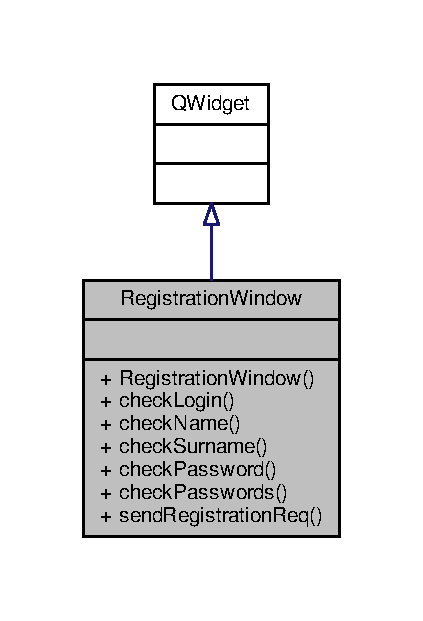
\includegraphics[width=203pt]{classRegistrationWindow__inherit__graph}
\end{center}
\end{figure}


Collaboration diagram for Registration\+Window\+:
\nopagebreak
\begin{figure}[H]
\begin{center}
\leavevmode
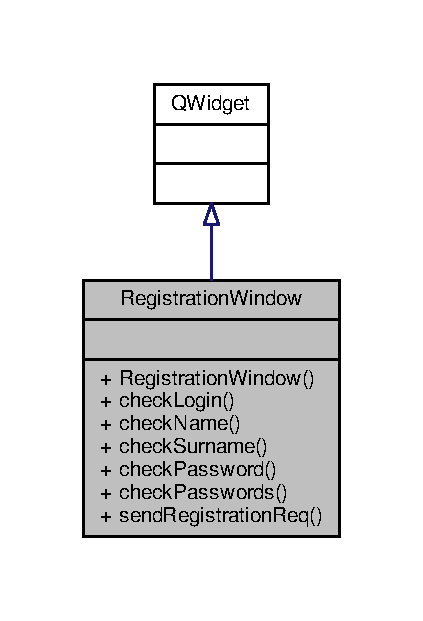
\includegraphics[width=203pt]{classRegistrationWindow__coll__graph}
\end{center}
\end{figure}
\subsection*{Public Types}
\begin{DoxyCompactItemize}
\item 
using \hyperlink{classRegistrationWindow_af737e72502243796bee87789c8b5b9ea}{String} = std\+::string
\end{DoxyCompactItemize}
\subsection*{Public Slots}
\begin{DoxyCompactItemize}
\item 
void \hyperlink{classRegistrationWindow_a054fcf4544f917e106aa6760f720d7b2}{check\+Login} (const Q\+String \&)
\item 
void \hyperlink{classRegistrationWindow_a26d58595ac8df47a0456878a80c45ffc}{check\+Name} (const Q\+String \&)
\item 
void \hyperlink{classRegistrationWindow_a6fc9f673b5e1d2fd15c9e12bfc0174b2}{check\+Surname} (const Q\+String \&)
\item 
void \hyperlink{classRegistrationWindow_a761ec197a38b335aaa5db06287361849}{check\+Password} (const Q\+String \&)
\item 
void \hyperlink{classRegistrationWindow_a6c3761195b00134d3ef4decf91ea76e7}{check\+Passwords} (const Q\+String \&)
\item 
void \hyperlink{classRegistrationWindow_a4344e4dafa6ab47e564c243b20a0c7a4}{send\+Registration\+Req} ()
\end{DoxyCompactItemize}
\subsection*{Public Member Functions}
\begin{DoxyCompactItemize}
\item 
\hyperlink{classRegistrationWindow_ac8876ad29199208fc8b8bd25863c9318}{Registration\+Window} (Controller \&)
\begin{DoxyCompactList}\small\item\em \hyperlink{classRegistrationWindow}{Registration\+Window} constructor for class \hyperlink{classRegistrationWindow}{Registration\+Window} which creates G\+UI for registration window. \end{DoxyCompactList}\end{DoxyCompactItemize}


\subsection{Detailed Description}
\hyperlink{classRegistrationWindow}{Registration\+Window} class which creates the G\+UI for login window. 

\subsection{Member Typedef Documentation}
\index{Registration\+Window@{Registration\+Window}!String@{String}}
\index{String@{String}!Registration\+Window@{Registration\+Window}}
\subsubsection[{\texorpdfstring{String}{String}}]{\setlength{\rightskip}{0pt plus 5cm}using {\bf Registration\+Window\+::\+String} =  std\+::string}\hypertarget{classRegistrationWindow_af737e72502243796bee87789c8b5b9ea}{}\label{classRegistrationWindow_af737e72502243796bee87789c8b5b9ea}


\subsection{Constructor \& Destructor Documentation}
\index{Registration\+Window@{Registration\+Window}!Registration\+Window@{Registration\+Window}}
\index{Registration\+Window@{Registration\+Window}!Registration\+Window@{Registration\+Window}}
\subsubsection[{\texorpdfstring{Registration\+Window(\+Controller \&)}{RegistrationWindow(Controller &)}}]{\setlength{\rightskip}{0pt plus 5cm}Registration\+Window\+::\+Registration\+Window (
\begin{DoxyParamCaption}
\item[{Controller \&}]{c}
\end{DoxyParamCaption}
)}\hypertarget{classRegistrationWindow_ac8876ad29199208fc8b8bd25863c9318}{}\label{classRegistrationWindow_ac8876ad29199208fc8b8bd25863c9318}


\hyperlink{classRegistrationWindow}{Registration\+Window} constructor for class \hyperlink{classRegistrationWindow}{Registration\+Window} which creates G\+UI for registration window. 


\begin{DoxyParams}{Parameters}
{\em is} & an initialized......??? \\
\hline
\end{DoxyParams}


\subsection{Member Function Documentation}
\index{Registration\+Window@{Registration\+Window}!check\+Login@{check\+Login}}
\index{check\+Login@{check\+Login}!Registration\+Window@{Registration\+Window}}
\subsubsection[{\texorpdfstring{check\+Login}{checkLogin}}]{\setlength{\rightskip}{0pt plus 5cm}void Registration\+Window\+::check\+Login (
\begin{DoxyParamCaption}
\item[{const Q\+String \&}]{qs}
\end{DoxyParamCaption}
)\hspace{0.3cm}{\ttfamily [slot]}}\hypertarget{classRegistrationWindow_a054fcf4544f917e106aa6760f720d7b2}{}\label{classRegistrationWindow_a054fcf4544f917e106aa6760f720d7b2}
\index{Registration\+Window@{Registration\+Window}!check\+Name@{check\+Name}}
\index{check\+Name@{check\+Name}!Registration\+Window@{Registration\+Window}}
\subsubsection[{\texorpdfstring{check\+Name}{checkName}}]{\setlength{\rightskip}{0pt plus 5cm}void Registration\+Window\+::check\+Name (
\begin{DoxyParamCaption}
\item[{const Q\+String \&}]{qs}
\end{DoxyParamCaption}
)\hspace{0.3cm}{\ttfamily [slot]}}\hypertarget{classRegistrationWindow_a26d58595ac8df47a0456878a80c45ffc}{}\label{classRegistrationWindow_a26d58595ac8df47a0456878a80c45ffc}
\index{Registration\+Window@{Registration\+Window}!check\+Password@{check\+Password}}
\index{check\+Password@{check\+Password}!Registration\+Window@{Registration\+Window}}
\subsubsection[{\texorpdfstring{check\+Password}{checkPassword}}]{\setlength{\rightskip}{0pt plus 5cm}void Registration\+Window\+::check\+Password (
\begin{DoxyParamCaption}
\item[{const Q\+String \&}]{qs}
\end{DoxyParamCaption}
)\hspace{0.3cm}{\ttfamily [slot]}}\hypertarget{classRegistrationWindow_a761ec197a38b335aaa5db06287361849}{}\label{classRegistrationWindow_a761ec197a38b335aaa5db06287361849}
\index{Registration\+Window@{Registration\+Window}!check\+Passwords@{check\+Passwords}}
\index{check\+Passwords@{check\+Passwords}!Registration\+Window@{Registration\+Window}}
\subsubsection[{\texorpdfstring{check\+Passwords}{checkPasswords}}]{\setlength{\rightskip}{0pt plus 5cm}void Registration\+Window\+::check\+Passwords (
\begin{DoxyParamCaption}
\item[{const Q\+String \&}]{qs}
\end{DoxyParamCaption}
)\hspace{0.3cm}{\ttfamily [slot]}}\hypertarget{classRegistrationWindow_a6c3761195b00134d3ef4decf91ea76e7}{}\label{classRegistrationWindow_a6c3761195b00134d3ef4decf91ea76e7}
\index{Registration\+Window@{Registration\+Window}!check\+Surname@{check\+Surname}}
\index{check\+Surname@{check\+Surname}!Registration\+Window@{Registration\+Window}}
\subsubsection[{\texorpdfstring{check\+Surname}{checkSurname}}]{\setlength{\rightskip}{0pt plus 5cm}void Registration\+Window\+::check\+Surname (
\begin{DoxyParamCaption}
\item[{const Q\+String \&}]{qs}
\end{DoxyParamCaption}
)\hspace{0.3cm}{\ttfamily [slot]}}\hypertarget{classRegistrationWindow_a6fc9f673b5e1d2fd15c9e12bfc0174b2}{}\label{classRegistrationWindow_a6fc9f673b5e1d2fd15c9e12bfc0174b2}
\index{Registration\+Window@{Registration\+Window}!send\+Registration\+Req@{send\+Registration\+Req}}
\index{send\+Registration\+Req@{send\+Registration\+Req}!Registration\+Window@{Registration\+Window}}
\subsubsection[{\texorpdfstring{send\+Registration\+Req}{sendRegistrationReq}}]{\setlength{\rightskip}{0pt plus 5cm}void Registration\+Window\+::send\+Registration\+Req (
\begin{DoxyParamCaption}
{}
\end{DoxyParamCaption}
)\hspace{0.3cm}{\ttfamily [slot]}}\hypertarget{classRegistrationWindow_a4344e4dafa6ab47e564c243b20a0c7a4}{}\label{classRegistrationWindow_a4344e4dafa6ab47e564c243b20a0c7a4}


The documentation for this class was generated from the following files\+:\begin{DoxyCompactItemize}
\item 
\hyperlink{RegistrationWindow_8hpp}{Registration\+Window.\+hpp}\item 
\hyperlink{RegistrationWindow_8cpp}{Registration\+Window.\+cpp}\end{DoxyCompactItemize}

\hypertarget{classServer}{}\section{Server Class Reference}
\label{classServer}\index{Server@{Server}}
\subsection*{Public Types}
\begin{DoxyCompactItemize}
\item 
using {\bfseries User} = \hyperlink{classServerUser}{Server\+User}\hypertarget{classServer_ae199c8a54f7743b0181ea5f48e50a69d}{}\label{classServer_ae199c8a54f7743b0181ea5f48e50a69d}

\item 
using {\bfseries Users} = std\+::multiset$<$ \hyperlink{classServerUser}{User} $>$\hypertarget{classServer_ab902a3e46b2e21d12d98abf605938220}{}\label{classServer_ab902a3e46b2e21d12d98abf605938220}

\item 
using {\bfseries User\+Iter} = Users\+::iterator\hypertarget{classServer_acef110486eb4a71d00b83283515779f1}{}\label{classServer_acef110486eb4a71d00b83283515779f1}

\item 
using {\bfseries Threads} = std\+::map$<$ S\+O\+C\+K\+ET, std\+::shared\+\_\+ptr$<$ pthread\+\_\+t $>$$>$\hypertarget{classServer_afdd32289149452b116ce1483d4fe18e6}{}\label{classServer_afdd32289149452b116ce1483d4fe18e6}

\item 
using {\bfseries String} = std\+::string\hypertarget{classServer_adb2fd27b9be87e7ba0206002a03e5998}{}\label{classServer_adb2fd27b9be87e7ba0206002a03e5998}

\end{DoxyCompactItemize}
\subsection*{Public Member Functions}
\begin{DoxyCompactItemize}
\item 
void {\bfseries run} ()\hypertarget{classServer_abb27d30b40a94326e3fd629d3b30b7d5}{}\label{classServer_abb27d30b40a94326e3fd629d3b30b7d5}

\item 
void {\bfseries handle\+Session} (S\+O\+C\+K\+ET)\hypertarget{classServer_a730cf1aeb7f2f7f173fb6e64164b7d05}{}\label{classServer_a730cf1aeb7f2f7f173fb6e64164b7d05}

\end{DoxyCompactItemize}


The documentation for this class was generated from the following files\+:\begin{DoxyCompactItemize}
\item 
core/Server.\+hpp\item 
core/Server.\+cpp\end{DoxyCompactItemize}

\hypertarget{classServerUser}{}\section{Server\+User Class Reference}
\label{classServerUser}\index{Server\+User@{Server\+User}}


.....  




{\ttfamily \#include $<$Server\+User.\+hpp$>$}

\subsection*{Public Types}
\begin{DoxyCompactItemize}
\item 
using {\bfseries String} = std\+::string\hypertarget{classServerUser_ad65781586abf71dbc8ceae3d0588f5a7}{}\label{classServerUser_ad65781586abf71dbc8ceae3d0588f5a7}

\item 
using {\bfseries Pending\+Messages} = std\+::list$<$ String $>$\hypertarget{classServerUser_a201c7266309a8f25e375f9560a3fc56b}{}\label{classServerUser_a201c7266309a8f25e375f9560a3fc56b}

\item 
using {\bfseries Size\+Type} = Pending\+Messages\+::size\+\_\+type\hypertarget{classServerUser_ab9bdd9958601b08bed543287a8869f3d}{}\label{classServerUser_ab9bdd9958601b08bed543287a8869f3d}

\item 
using {\bfseries P\+Messages\+Ptr} = std\+::shared\+\_\+ptr$<$ Pending\+Messages $>$\hypertarget{classServerUser_ab4b74b95dcdcd0d2be56c2becd825a90}{}\label{classServerUser_ab4b74b95dcdcd0d2be56c2becd825a90}

\end{DoxyCompactItemize}
\subsection*{Public Member Functions}
\begin{DoxyCompactItemize}
\item 
\hyperlink{classServerUser_aabd76de5124914eb323ea964b50595c5}{Server\+User} ()
\begin{DoxyCompactList}\small\item\em ... \end{DoxyCompactList}\item 
\hyperlink{classServerUser_a3cca664c936634392a5246c422442a49}{Server\+User} (const S\+O\+C\+K\+ET, const String \&, const String \&, const String \&, const String \&, const bool)
\begin{DoxyCompactList}\small\item\em .... \end{DoxyCompactList}\item 
\hyperlink{classServerUser_a01a83ba512b3aabbfd47dd4b72531255}{Server\+User} (const S\+O\+C\+K\+ET)
\begin{DoxyCompactList}\small\item\em .... \end{DoxyCompactList}\item 
String \hyperlink{classServerUser_a7b0aa031af58d004834d15212e439ef1}{to\+String} () const 
\begin{DoxyCompactList}\small\item\em .... \end{DoxyCompactList}\item 
String \hyperlink{classServerUser_a7822915335144b12ad6793002a978c85}{to\+String\+Log} () const 
\begin{DoxyCompactList}\small\item\em ..... \end{DoxyCompactList}\item 
bool \hyperlink{classServerUser_aeed52246e162281d7a1c38cd9fe2eb93}{from\+String} (String \&)
\begin{DoxyCompactList}\small\item\em .... \end{DoxyCompactList}\item 
bool \hyperlink{classServerUser_a0bc2c243319fe618849f8c4842c820c0}{from\+String} (String \&, int)
\begin{DoxyCompactList}\small\item\em .... \end{DoxyCompactList}\item 
S\+O\+C\+K\+ET \hyperlink{classServerUser_aa260c021d44bce338061b2ffe187c260}{get\+Socket} () const 
\begin{DoxyCompactList}\small\item\em ... \end{DoxyCompactList}\item 
String \hyperlink{classServerUser_a4ace9b03d2dcde07b616468608bc1ae0}{get\+Login} () const 
\begin{DoxyCompactList}\small\item\em .... \end{DoxyCompactList}\item 
String \hyperlink{classServerUser_a763e23bc60062a9f216af69cc003a6d8}{get\+Name} () const 
\begin{DoxyCompactList}\small\item\em .... \end{DoxyCompactList}\item 
String \hyperlink{classServerUser_a65791cc9ca96585bde4483fb11d97adb}{get\+Surname} () const 
\begin{DoxyCompactList}\small\item\em ... \end{DoxyCompactList}\item 
String \hyperlink{classServerUser_a46ee509027d923a27e644f4fb891231b}{get\+Password} () const 
\begin{DoxyCompactList}\small\item\em ... \end{DoxyCompactList}\item 
bool \hyperlink{classServerUser_a2ec1eff8b6b0d16b71ac0bae8953af22}{get\+Status} () const 
\begin{DoxyCompactList}\small\item\em ... \end{DoxyCompactList}\item 
void \hyperlink{classServerUser_a50305db89103b56b3205be2e8fd328cc}{set\+Socket} (const S\+O\+C\+K\+ET) const 
\begin{DoxyCompactList}\small\item\em .... \end{DoxyCompactList}\item 
void \hyperlink{classServerUser_a29f0ed0f022e7051aaf429dfe6ce42b3}{set\+Status} (const bool) const 
\begin{DoxyCompactList}\small\item\em .... \end{DoxyCompactList}\item 
Size\+Type \hyperlink{classServerUser_aaa586562b5a35b39c187728f32c36dae}{messages\+Count} () const 
\begin{DoxyCompactList}\small\item\em ... \end{DoxyCompactList}\item 
void \hyperlink{classServerUser_ae6cf777a460e07d563b4e14ef9baf131}{set\+P\+Messages} (P\+Messages\+Ptr) const 
\begin{DoxyCompactList}\small\item\em ..... \end{DoxyCompactList}\item 
P\+Messages\+Ptr \hyperlink{classServerUser_ac6a83ceae296cebeba44b83e93050a53}{get\+P\+Messages} () const 
\begin{DoxyCompactList}\small\item\em ...... \end{DoxyCompactList}\item 
void \hyperlink{classServerUser_a922bc75b62a9eeeab0c5bb4433f8a34e}{close\+Socket} () const 
\begin{DoxyCompactList}\small\item\em .... \end{DoxyCompactList}\item 
bool {\bfseries operator$<$} (const \hyperlink{classServerUser}{Server\+User} \&) const \hypertarget{classServerUser_adb3605ca08c5cf0ffe6dcfb3d108f744}{}\label{classServerUser_adb3605ca08c5cf0ffe6dcfb3d108f744}

\item 
void {\bfseries operator=} (const \hyperlink{classServerUser}{Server\+User} \&)\hypertarget{classServerUser_a2a52373517ea958408232ab06ff8610f}{}\label{classServerUser_a2a52373517ea958408232ab06ff8610f}

\item 
\hyperlink{classServerUser}{Server\+User} $\ast$ \hyperlink{classServerUser_ae6eb28131e727129e8797117a1a4421d}{get\+Pointer} () const 
\begin{DoxyCompactList}\small\item\em ..... \end{DoxyCompactList}\end{DoxyCompactItemize}


\subsection{Detailed Description}
..... 

\subsection{Constructor \& Destructor Documentation}
\index{Server\+User@{Server\+User}!Server\+User@{Server\+User}}
\index{Server\+User@{Server\+User}!Server\+User@{Server\+User}}
\subsubsection[{\texorpdfstring{Server\+User()}{ServerUser()}}]{\setlength{\rightskip}{0pt plus 5cm}Server\+User\+::\+Server\+User (
\begin{DoxyParamCaption}
{}
\end{DoxyParamCaption}
)}\hypertarget{classServerUser_aabd76de5124914eb323ea964b50595c5}{}\label{classServerUser_aabd76de5124914eb323ea964b50595c5}


... 


\begin{DoxyParams}{Parameters}
{\em no} & parametrs \\
\hline
\end{DoxyParams}
\index{Server\+User@{Server\+User}!Server\+User@{Server\+User}}
\index{Server\+User@{Server\+User}!Server\+User@{Server\+User}}
\subsubsection[{\texorpdfstring{Server\+User(const S\+O\+C\+K\+E\+T, const String \&, const String \&, const String \&, const String \&, const bool)}{ServerUser(const SOCKET, const String &, const String &, const String &, const String &, const bool)}}]{\setlength{\rightskip}{0pt plus 5cm}Server\+User\+::\+Server\+User (
\begin{DoxyParamCaption}
\item[{const S\+O\+C\+K\+ET}]{sock, }
\item[{const String \&}]{login, }
\item[{const String \&}]{name, }
\item[{const String \&}]{surname, }
\item[{const String \&}]{password, }
\item[{const bool}]{st}
\end{DoxyParamCaption}
)}\hypertarget{classServerUser_a3cca664c936634392a5246c422442a49}{}\label{classServerUser_a3cca664c936634392a5246c422442a49}


.... 


\begin{DoxyParams}{Parameters}
{\em is} & an initialized.... ?? \\
\hline
\end{DoxyParams}
\index{Server\+User@{Server\+User}!Server\+User@{Server\+User}}
\index{Server\+User@{Server\+User}!Server\+User@{Server\+User}}
\subsubsection[{\texorpdfstring{Server\+User(const S\+O\+C\+K\+E\+T)}{ServerUser(const SOCKET)}}]{\setlength{\rightskip}{0pt plus 5cm}Server\+User\+::\+Server\+User (
\begin{DoxyParamCaption}
\item[{const S\+O\+C\+K\+ET}]{sock}
\end{DoxyParamCaption}
)\hspace{0.3cm}{\ttfamily [explicit]}}\hypertarget{classServerUser_a01a83ba512b3aabbfd47dd4b72531255}{}\label{classServerUser_a01a83ba512b3aabbfd47dd4b72531255}


.... 


\begin{DoxyParams}{Parameters}
{\em is} & an initialized.... ?? \\
\hline
\end{DoxyParams}


\subsection{Member Function Documentation}
\index{Server\+User@{Server\+User}!close\+Socket@{close\+Socket}}
\index{close\+Socket@{close\+Socket}!Server\+User@{Server\+User}}
\subsubsection[{\texorpdfstring{close\+Socket() const }{closeSocket() const }}]{\setlength{\rightskip}{0pt plus 5cm}void Server\+User\+::close\+Socket (
\begin{DoxyParamCaption}
{}
\end{DoxyParamCaption}
) const}\hypertarget{classServerUser_a922bc75b62a9eeeab0c5bb4433f8a34e}{}\label{classServerUser_a922bc75b62a9eeeab0c5bb4433f8a34e}


.... 


\begin{DoxyParams}{Parameters}
{\em no} & parametrs \\
\hline
\end{DoxyParams}
\begin{DoxyReturn}{Returns}
void 
\end{DoxyReturn}
\index{Server\+User@{Server\+User}!from\+String@{from\+String}}
\index{from\+String@{from\+String}!Server\+User@{Server\+User}}
\subsubsection[{\texorpdfstring{from\+String(\+String \&)}{fromString(String &)}}]{\setlength{\rightskip}{0pt plus 5cm}bool Server\+User\+::from\+String (
\begin{DoxyParamCaption}
\item[{String \&}]{str}
\end{DoxyParamCaption}
)}\hypertarget{classServerUser_aeed52246e162281d7a1c38cd9fe2eb93}{}\label{classServerUser_aeed52246e162281d7a1c38cd9fe2eb93}


.... 


\begin{DoxyParams}{Parameters}
{\em is} & an initialized.... ?? \\
\hline
\end{DoxyParams}
\begin{DoxyReturn}{Returns}
bool 
\end{DoxyReturn}
\index{Server\+User@{Server\+User}!from\+String@{from\+String}}
\index{from\+String@{from\+String}!Server\+User@{Server\+User}}
\subsubsection[{\texorpdfstring{from\+String(\+String \&, int)}{fromString(String &, int)}}]{\setlength{\rightskip}{0pt plus 5cm}bool Server\+User\+::from\+String (
\begin{DoxyParamCaption}
\item[{String \&}]{str, }
\item[{int}]{}
\end{DoxyParamCaption}
)}\hypertarget{classServerUser_a0bc2c243319fe618849f8c4842c820c0}{}\label{classServerUser_a0bc2c243319fe618849f8c4842c820c0}


.... 


\begin{DoxyParams}{Parameters}
{\em is} & an initialized.... ?? \\
\hline
\end{DoxyParams}
\begin{DoxyReturn}{Returns}
bool 
\end{DoxyReturn}
\index{Server\+User@{Server\+User}!get\+Login@{get\+Login}}
\index{get\+Login@{get\+Login}!Server\+User@{Server\+User}}
\subsubsection[{\texorpdfstring{get\+Login() const }{getLogin() const }}]{\setlength{\rightskip}{0pt plus 5cm}String Server\+User\+::get\+Login (
\begin{DoxyParamCaption}
{}
\end{DoxyParamCaption}
) const}\hypertarget{classServerUser_a4ace9b03d2dcde07b616468608bc1ae0}{}\label{classServerUser_a4ace9b03d2dcde07b616468608bc1ae0}


.... 


\begin{DoxyParams}{Parameters}
{\em no} & parametrs \\
\hline
\end{DoxyParams}
\begin{DoxyReturn}{Returns}
String 
\end{DoxyReturn}
\index{Server\+User@{Server\+User}!get\+Name@{get\+Name}}
\index{get\+Name@{get\+Name}!Server\+User@{Server\+User}}
\subsubsection[{\texorpdfstring{get\+Name() const }{getName() const }}]{\setlength{\rightskip}{0pt plus 5cm}String Server\+User\+::get\+Name (
\begin{DoxyParamCaption}
{}
\end{DoxyParamCaption}
) const}\hypertarget{classServerUser_a763e23bc60062a9f216af69cc003a6d8}{}\label{classServerUser_a763e23bc60062a9f216af69cc003a6d8}


.... 


\begin{DoxyParams}{Parameters}
{\em no} & parametrs \\
\hline
\end{DoxyParams}
\begin{DoxyReturn}{Returns}
String 
\end{DoxyReturn}
\index{Server\+User@{Server\+User}!get\+Password@{get\+Password}}
\index{get\+Password@{get\+Password}!Server\+User@{Server\+User}}
\subsubsection[{\texorpdfstring{get\+Password() const }{getPassword() const }}]{\setlength{\rightskip}{0pt plus 5cm}String Server\+User\+::get\+Password (
\begin{DoxyParamCaption}
{}
\end{DoxyParamCaption}
) const}\hypertarget{classServerUser_a46ee509027d923a27e644f4fb891231b}{}\label{classServerUser_a46ee509027d923a27e644f4fb891231b}


... 


\begin{DoxyParams}{Parameters}
{\em no} & parametrs \\
\hline
\end{DoxyParams}
\begin{DoxyReturn}{Returns}
String 
\end{DoxyReturn}
\index{Server\+User@{Server\+User}!get\+P\+Messages@{get\+P\+Messages}}
\index{get\+P\+Messages@{get\+P\+Messages}!Server\+User@{Server\+User}}
\subsubsection[{\texorpdfstring{get\+P\+Messages() const }{getPMessages() const }}]{\setlength{\rightskip}{0pt plus 5cm}Server\+User\+::\+P\+Messages\+Ptr Server\+User\+::get\+P\+Messages (
\begin{DoxyParamCaption}
{}
\end{DoxyParamCaption}
) const}\hypertarget{classServerUser_ac6a83ceae296cebeba44b83e93050a53}{}\label{classServerUser_ac6a83ceae296cebeba44b83e93050a53}


...... 


\begin{DoxyParams}{Parameters}
{\em no} & parametrs \\
\hline
\end{DoxyParams}
\begin{DoxyReturn}{Returns}
.... 
\end{DoxyReturn}
\index{Server\+User@{Server\+User}!get\+Pointer@{get\+Pointer}}
\index{get\+Pointer@{get\+Pointer}!Server\+User@{Server\+User}}
\subsubsection[{\texorpdfstring{get\+Pointer() const }{getPointer() const }}]{\setlength{\rightskip}{0pt plus 5cm}{\bf Server\+User} $\ast$ Server\+User\+::get\+Pointer (
\begin{DoxyParamCaption}
{}
\end{DoxyParamCaption}
) const}\hypertarget{classServerUser_ae6eb28131e727129e8797117a1a4421d}{}\label{classServerUser_ae6eb28131e727129e8797117a1a4421d}


..... 


\begin{DoxyParams}{Parameters}
{\em no} & parametrs \\
\hline
\end{DoxyParams}
\begin{DoxyReturn}{Returns}
.... 
\end{DoxyReturn}
\index{Server\+User@{Server\+User}!get\+Socket@{get\+Socket}}
\index{get\+Socket@{get\+Socket}!Server\+User@{Server\+User}}
\subsubsection[{\texorpdfstring{get\+Socket() const }{getSocket() const }}]{\setlength{\rightskip}{0pt plus 5cm}S\+O\+C\+K\+ET Server\+User\+::get\+Socket (
\begin{DoxyParamCaption}
{}
\end{DoxyParamCaption}
) const}\hypertarget{classServerUser_aa260c021d44bce338061b2ffe187c260}{}\label{classServerUser_aa260c021d44bce338061b2ffe187c260}


... 


\begin{DoxyParams}{Parameters}
{\em no} & parametrs \\
\hline
\end{DoxyParams}
\begin{DoxyReturn}{Returns}
... 
\end{DoxyReturn}
\index{Server\+User@{Server\+User}!get\+Status@{get\+Status}}
\index{get\+Status@{get\+Status}!Server\+User@{Server\+User}}
\subsubsection[{\texorpdfstring{get\+Status() const }{getStatus() const }}]{\setlength{\rightskip}{0pt plus 5cm}bool Server\+User\+::get\+Status (
\begin{DoxyParamCaption}
{}
\end{DoxyParamCaption}
) const}\hypertarget{classServerUser_a2ec1eff8b6b0d16b71ac0bae8953af22}{}\label{classServerUser_a2ec1eff8b6b0d16b71ac0bae8953af22}


... 


\begin{DoxyParams}{Parameters}
{\em no} & parametrs \\
\hline
\end{DoxyParams}
\begin{DoxyReturn}{Returns}
bool 
\end{DoxyReturn}
\index{Server\+User@{Server\+User}!get\+Surname@{get\+Surname}}
\index{get\+Surname@{get\+Surname}!Server\+User@{Server\+User}}
\subsubsection[{\texorpdfstring{get\+Surname() const }{getSurname() const }}]{\setlength{\rightskip}{0pt plus 5cm}String Server\+User\+::get\+Surname (
\begin{DoxyParamCaption}
{}
\end{DoxyParamCaption}
) const}\hypertarget{classServerUser_a65791cc9ca96585bde4483fb11d97adb}{}\label{classServerUser_a65791cc9ca96585bde4483fb11d97adb}


... 


\begin{DoxyParams}{Parameters}
{\em no} & parametrs \\
\hline
\end{DoxyParams}
\begin{DoxyReturn}{Returns}
String 
\end{DoxyReturn}
\index{Server\+User@{Server\+User}!messages\+Count@{messages\+Count}}
\index{messages\+Count@{messages\+Count}!Server\+User@{Server\+User}}
\subsubsection[{\texorpdfstring{messages\+Count() const }{messagesCount() const }}]{\setlength{\rightskip}{0pt plus 5cm}Server\+User\+::\+Size\+Type Server\+User\+::messages\+Count (
\begin{DoxyParamCaption}
{}
\end{DoxyParamCaption}
) const}\hypertarget{classServerUser_aaa586562b5a35b39c187728f32c36dae}{}\label{classServerUser_aaa586562b5a35b39c187728f32c36dae}


... 


\begin{DoxyParams}{Parameters}
{\em no} & parametrs \\
\hline
\end{DoxyParams}
\begin{DoxyReturn}{Returns}
.... 
\end{DoxyReturn}
\index{Server\+User@{Server\+User}!set\+P\+Messages@{set\+P\+Messages}}
\index{set\+P\+Messages@{set\+P\+Messages}!Server\+User@{Server\+User}}
\subsubsection[{\texorpdfstring{set\+P\+Messages(\+P\+Messages\+Ptr) const }{setPMessages(PMessagesPtr) const }}]{\setlength{\rightskip}{0pt plus 5cm}void Server\+User\+::set\+P\+Messages (
\begin{DoxyParamCaption}
\item[{P\+Messages\+Ptr}]{pm}
\end{DoxyParamCaption}
) const}\hypertarget{classServerUser_ae6cf777a460e07d563b4e14ef9baf131}{}\label{classServerUser_ae6cf777a460e07d563b4e14ef9baf131}


..... 


\begin{DoxyParams}{Parameters}
{\em is} & an initialized.... ?? \\
\hline
\end{DoxyParams}
\begin{DoxyReturn}{Returns}
void 
\end{DoxyReturn}
\index{Server\+User@{Server\+User}!set\+Socket@{set\+Socket}}
\index{set\+Socket@{set\+Socket}!Server\+User@{Server\+User}}
\subsubsection[{\texorpdfstring{set\+Socket(const S\+O\+C\+K\+E\+T) const }{setSocket(const SOCKET) const }}]{\setlength{\rightskip}{0pt plus 5cm}void Server\+User\+::set\+Socket (
\begin{DoxyParamCaption}
\item[{const S\+O\+C\+K\+ET}]{s}
\end{DoxyParamCaption}
) const}\hypertarget{classServerUser_a50305db89103b56b3205be2e8fd328cc}{}\label{classServerUser_a50305db89103b56b3205be2e8fd328cc}


.... 


\begin{DoxyParams}{Parameters}
{\em is} & an initialized.... ?? \\
\hline
\end{DoxyParams}
\begin{DoxyReturn}{Returns}
void 
\end{DoxyReturn}
\index{Server\+User@{Server\+User}!set\+Status@{set\+Status}}
\index{set\+Status@{set\+Status}!Server\+User@{Server\+User}}
\subsubsection[{\texorpdfstring{set\+Status(const bool) const }{setStatus(const bool) const }}]{\setlength{\rightskip}{0pt plus 5cm}void Server\+User\+::set\+Status (
\begin{DoxyParamCaption}
\item[{const bool}]{st}
\end{DoxyParamCaption}
) const}\hypertarget{classServerUser_a29f0ed0f022e7051aaf429dfe6ce42b3}{}\label{classServerUser_a29f0ed0f022e7051aaf429dfe6ce42b3}


.... 


\begin{DoxyParams}{Parameters}
{\em is} & an initialized.... ?? \\
\hline
\end{DoxyParams}
\begin{DoxyReturn}{Returns}
void 
\end{DoxyReturn}
\index{Server\+User@{Server\+User}!to\+String@{to\+String}}
\index{to\+String@{to\+String}!Server\+User@{Server\+User}}
\subsubsection[{\texorpdfstring{to\+String() const }{toString() const }}]{\setlength{\rightskip}{0pt plus 5cm}String Server\+User\+::to\+String (
\begin{DoxyParamCaption}
{}
\end{DoxyParamCaption}
) const}\hypertarget{classServerUser_a7b0aa031af58d004834d15212e439ef1}{}\label{classServerUser_a7b0aa031af58d004834d15212e439ef1}


.... 


\begin{DoxyParams}{Parameters}
{\em no} & parametrs \\
\hline
\end{DoxyParams}
\begin{DoxyReturn}{Returns}
String 
\end{DoxyReturn}
\index{Server\+User@{Server\+User}!to\+String\+Log@{to\+String\+Log}}
\index{to\+String\+Log@{to\+String\+Log}!Server\+User@{Server\+User}}
\subsubsection[{\texorpdfstring{to\+String\+Log() const }{toStringLog() const }}]{\setlength{\rightskip}{0pt plus 5cm}String Server\+User\+::to\+String\+Log (
\begin{DoxyParamCaption}
{}
\end{DoxyParamCaption}
) const}\hypertarget{classServerUser_a7822915335144b12ad6793002a978c85}{}\label{classServerUser_a7822915335144b12ad6793002a978c85}


..... 


\begin{DoxyParams}{Parameters}
{\em no} & parametrs \\
\hline
\end{DoxyParams}
\begin{DoxyReturn}{Returns}
String 
\end{DoxyReturn}


The documentation for this class was generated from the following files\+:\begin{DoxyCompactItemize}
\item 
core/\hyperlink{ServerUser_8hpp}{Server\+User.\+hpp}\item 
core/Server\+User.\+cpp\end{DoxyCompactItemize}

\hypertarget{classTransportLayer}{}\section{Transport\+Layer Class Reference}
\label{classTransportLayer}\index{Transport\+Layer@{Transport\+Layer}}


....  




{\ttfamily \#include $<$Transport\+Layer.\+hpp$>$}

\subsection*{Classes}
\begin{DoxyCompactItemize}
\item 
class \hyperlink{classTransportLayer_1_1Iterator}{Iterator}
\begin{DoxyCompactList}\small\item\em ..... \end{DoxyCompactList}\end{DoxyCompactItemize}
\subsection*{Public Types}
\begin{DoxyCompactItemize}
\item 
using {\bfseries String} = std\+::string\hypertarget{classTransportLayer_abb9ea2afa20f4277013ab8b9d870f3e4}{}\label{classTransportLayer_abb9ea2afa20f4277013ab8b9d870f3e4}

\item 
using {\bfseries Message} = std\+::shared\+\_\+ptr$<$ String $>$\hypertarget{classTransportLayer_af43e07ebb1a1725bc6f13fd4cc69d429}{}\label{classTransportLayer_af43e07ebb1a1725bc6f13fd4cc69d429}

\item 
using {\bfseries Messages} = std\+::list$<$ Message $>$\hypertarget{classTransportLayer_a0ff31cb0269d468ed1af9b9a6ecd34c4}{}\label{classTransportLayer_a0ff31cb0269d468ed1af9b9a6ecd34c4}

\end{DoxyCompactItemize}
\subsection*{Public Member Functions}
\begin{DoxyCompactItemize}
\item 
\hyperlink{classTransportLayer_1_1Iterator}{Iterator} {\bfseries begin} ()\hypertarget{classTransportLayer_a635826c2399e9ff851bed57e6829948b}{}\label{classTransportLayer_a635826c2399e9ff851bed57e6829948b}

\item 
\hyperlink{classTransportLayer_1_1Iterator}{Iterator} {\bfseries end} ()\hypertarget{classTransportLayer_aba0bbf660b9a5f146ebccfa49d42809c}{}\label{classTransportLayer_aba0bbf660b9a5f146ebccfa49d42809c}

\item 
void {\bfseries process\+Message} (char $\ast$)\hypertarget{classTransportLayer_aa997123a0b253f07a66f73d9388111d6}{}\label{classTransportLayer_aa997123a0b253f07a66f73d9388111d6}

\item 
void {\bfseries clear} ()\hypertarget{classTransportLayer_a92828c3ac48c25dfdf166e9a0907285e}{}\label{classTransportLayer_a92828c3ac48c25dfdf166e9a0907285e}

\end{DoxyCompactItemize}


\subsection{Detailed Description}
.... 

The documentation for this class was generated from the following files\+:\begin{DoxyCompactItemize}
\item 
core/\hyperlink{TransportLayer_8hpp}{Transport\+Layer.\+hpp}\item 
core/Transport\+Layer.\+cpp\end{DoxyCompactItemize}

\hypertarget{classWriteBox}{}\section{Write\+Box Class Reference}
\label{classWriteBox}\index{Write\+Box@{Write\+Box}}


....  




{\ttfamily \#include $<$Write\+Box.\+hpp$>$}



Inheritance diagram for Write\+Box\+:
% FIG 0


Collaboration diagram for Write\+Box\+:
% FIG 1
\subsection*{Public Types}
\begin{DoxyCompactItemize}
\item 
using {\bfseries String} = std\+::string\hypertarget{classWriteBox_a64feff0630b723ed37022278a248d206}{}\label{classWriteBox_a64feff0630b723ed37022278a248d206}

\end{DoxyCompactItemize}
\subsection*{Public Slots}
\begin{DoxyCompactItemize}
\item 
void {\bfseries send\+Message} ()\hypertarget{classWriteBox_a94b304997cbaf9b3f4dc1975d60f421f}{}\label{classWriteBox_a94b304997cbaf9b3f4dc1975d60f421f}

\end{DoxyCompactItemize}
\subsection*{Public Member Functions}
\begin{DoxyCompactItemize}
\item 
\hyperlink{classWriteBox_aed152f91f59c5fe8a3de845ee615c601}{Write\+Box} (\hyperlink{classMainWindow}{Main\+Window} \&)
\begin{DoxyCompactList}\small\item\em .... \end{DoxyCompactList}\item 
Q\+Layout $\ast$ \hyperlink{classWriteBox_a0264739b6b85d865237055b1b26061dd}{get\+Write\+Box} ()
\begin{DoxyCompactList}\small\item\em .... \end{DoxyCompactList}\end{DoxyCompactItemize}


\subsection{Detailed Description}
.... 

\subsection{Constructor \& Destructor Documentation}
\index{Write\+Box@{Write\+Box}!Write\+Box@{Write\+Box}}
\index{Write\+Box@{Write\+Box}!Write\+Box@{Write\+Box}}
\subsubsection[{\texorpdfstring{Write\+Box(\+Main\+Window \&)}{WriteBox(MainWindow &)}}]{\setlength{\rightskip}{0pt plus 5cm}Write\+Box\+::\+Write\+Box (
\begin{DoxyParamCaption}
\item[{{\bf Main\+Window} \&}]{mw}
\end{DoxyParamCaption}
)}\hypertarget{classWriteBox_aed152f91f59c5fe8a3de845ee615c601}{}\label{classWriteBox_aed152f91f59c5fe8a3de845ee615c601}


.... 


\begin{DoxyParams}{Parameters}
{\em ....} & \\
\hline
\end{DoxyParams}


\subsection{Member Function Documentation}
\index{Write\+Box@{Write\+Box}!get\+Write\+Box@{get\+Write\+Box}}
\index{get\+Write\+Box@{get\+Write\+Box}!Write\+Box@{Write\+Box}}
\subsubsection[{\texorpdfstring{get\+Write\+Box()}{getWriteBox()}}]{\setlength{\rightskip}{0pt plus 5cm}Q\+Layout $\ast$ Write\+Box\+::get\+Write\+Box (
\begin{DoxyParamCaption}
{}
\end{DoxyParamCaption}
)}\hypertarget{classWriteBox_a0264739b6b85d865237055b1b26061dd}{}\label{classWriteBox_a0264739b6b85d865237055b1b26061dd}


.... 


\begin{DoxyParams}{Parameters}
{\em no} & parametrs \\
\hline
\end{DoxyParams}
\begin{DoxyReturn}{Returns}
.... 
\end{DoxyReturn}


The documentation for this class was generated from the following files\+:\begin{DoxyCompactItemize}
\item 
gui/\+Main\+Window/Write\+Box.\+hpp\item 
gui/\+Main\+Window/Write\+Box.\+cpp\end{DoxyCompactItemize}

\chapter{File Documentation}
\hypertarget{Client_8hpp}{}\section{core/\+Client.hpp File Reference}
\label{Client_8hpp}\index{core/\+Client.\+hpp@{core/\+Client.\+hpp}}


....  


{\ttfamily \#include \char`\"{}Includes.\+hpp\char`\"{}}\\*
{\ttfamily \#include \char`\"{}D\+B\+Controller.\+hpp\char`\"{}}\\*
{\ttfamily \#include \char`\"{}Transport\+Layer.\+hpp\char`\"{}}\\*
Include dependency graph for Client.\+hpp\+:

\hypertarget{ClientUser_8hpp}{}\section{core/\+Client\+User.hpp File Reference}
\label{ClientUser_8hpp}\index{core/\+Client\+User.\+hpp@{core/\+Client\+User.\+hpp}}
{\ttfamily \#include $<$string$>$}\\*
{\ttfamily \#include $<$list$>$}\\*
{\ttfamily \#include $<$memory$>$}\\*
{\ttfamily \#include \char`\"{}Extract\+Word.\+hpp\char`\"{}}\\*
Include dependency graph for Client\+User.\+hpp\+:
% FIG 0
This graph shows which files directly or indirectly include this file\+:
% FIG 1
\subsection*{Classes}
\begin{DoxyCompactItemize}
\item 
class \hyperlink{classClientUser}{Client\+User}
\begin{DoxyCompactList}\small\item\em \hyperlink{classClientUser}{Client\+User} Class. \end{DoxyCompactList}\end{DoxyCompactItemize}


\subsection{Detailed Description}
\begin{DoxyAuthor}{Author}
G\+RI Team 
\end{DoxyAuthor}
\begin{DoxyDate}{Date}
06/21/2017 
\end{DoxyDate}
\begin{DoxyVersion}{Version}
1.\+0 
\end{DoxyVersion}

\hypertarget{Controller_8hpp}{}\section{core/\+Controller.hpp File Reference}
\label{Controller_8hpp}\index{core/\+Controller.\+hpp@{core/\+Controller.\+hpp}}
{\ttfamily \#include \char`\"{}Client.\+hpp\char`\"{}}\\*
{\ttfamily \#include \char`\"{}Client\+User.\+hpp\char`\"{}}\\*
{\ttfamily \#include \char`\"{}D\+B\+Controller.\+hpp\char`\"{}}\\*
{\ttfamily \#include \char`\"{}Input\+Validator.\+hpp\char`\"{}}\\*
{\ttfamily \#include \char`\"{}Transport\+Layer.\+hpp\char`\"{}}\\*
Include dependency graph for Controller.\+hpp\+:
% FIG 0
This graph shows which files directly or indirectly include this file\+:
% FIG 1
\subsection*{Classes}
\begin{DoxyCompactItemize}
\item 
class \hyperlink{classController}{Controller}
\item 
class \hyperlink{classController_1_1InputReader}{Controller\+::\+Input\+Reader}
\end{DoxyCompactItemize}
\subsection*{Functions}
\begin{DoxyCompactItemize}
\item 
void $\ast$ {\bfseries read\+Message} (void $\ast$)\hypertarget{Controller_8hpp_a4f8c0af155366aa614f0c050c8b88068}{}\label{Controller_8hpp_a4f8c0af155366aa614f0c050c8b88068}

\item 
void $\ast$ {\bfseries handle\+Session} (void $\ast$)\hypertarget{Controller_8hpp_a9d248705aaaac00e0359e3a77e25c846}{}\label{Controller_8hpp_a9d248705aaaac00e0359e3a77e25c846}

\end{DoxyCompactItemize}


\subsection{Detailed Description}
\begin{DoxyAuthor}{Author}
G\+RI Team 
\end{DoxyAuthor}
\begin{DoxyDate}{Date}
06/22/2017 
\end{DoxyDate}
\begin{DoxyVersion}{Version}
1.\+0 
\end{DoxyVersion}

\hypertarget{ServerUser_8hpp}{}\section{core/\+Server\+User.hpp File Reference}
\label{ServerUser_8hpp}\index{core/\+Server\+User.\+hpp@{core/\+Server\+User.\+hpp}}


....  


{\ttfamily \#include \char`\"{}Extract\+Word.\+hpp\char`\"{}}\\*
{\ttfamily \#include \char`\"{}Includes.\+hpp\char`\"{}}\\*
Include dependency graph for Server\+User.\+hpp\+:
% FIG 0
This graph shows which files directly or indirectly include this file\+:
% FIG 1
\subsection*{Classes}
\begin{DoxyCompactItemize}
\item 
class \hyperlink{classServerUser}{Server\+User}
\begin{DoxyCompactList}\small\item\em ..... \end{DoxyCompactList}\end{DoxyCompactItemize}


\subsection{Detailed Description}
.... 

\begin{DoxyAuthor}{Author}
G\+RI Team 
\end{DoxyAuthor}
\begin{DoxyDate}{Date}
06/22/2017 
\end{DoxyDate}
\begin{DoxyVersion}{Version}
1.\+0 
\end{DoxyVersion}

\hypertarget{TransportLayer_8hpp}{}\section{core/\+Transport\+Layer.hpp File Reference}
\label{TransportLayer_8hpp}\index{core/\+Transport\+Layer.\+hpp@{core/\+Transport\+Layer.\+hpp}}


...  


{\ttfamily \#include $<$string$>$}\\*
{\ttfamily \#include $<$list$>$}\\*
{\ttfamily \#include $<$memory$>$}\\*
{\ttfamily \#include $<$iterator$>$}\\*
{\ttfamily \#include \char`\"{}Extract\+Word.\+hpp\char`\"{}}\\*
Include dependency graph for Transport\+Layer.\+hpp\+:
% FIG 0
This graph shows which files directly or indirectly include this file\+:
% FIG 1
\subsection*{Classes}
\begin{DoxyCompactItemize}
\item 
class \hyperlink{classTransportLayer}{Transport\+Layer}
\begin{DoxyCompactList}\small\item\em .... \end{DoxyCompactList}\item 
class \hyperlink{classTransportLayer_1_1Iterator}{Transport\+Layer\+::\+Iterator}
\begin{DoxyCompactList}\small\item\em ..... \end{DoxyCompactList}\end{DoxyCompactItemize}


\subsection{Detailed Description}
... 

\begin{DoxyAuthor}{Author}
G\+RI Team 
\end{DoxyAuthor}
\begin{DoxyDate}{Date}
06/22/2017 
\end{DoxyDate}
\begin{DoxyVersion}{Version}
1.\+0 
\end{DoxyVersion}

\hypertarget{LoginWindow_8hpp}{}\section{Login\+Window.\+hpp File Reference}
\label{LoginWindow_8hpp}\index{Login\+Window.\+hpp@{Login\+Window.\+hpp}}


\hyperlink{LoginWindow_8hpp}{Login\+Window.\+hpp} creating a G\+UI for login window and connection for checking the login password.  


{\ttfamily \#include $<$Q\+Object$>$}\\*
{\ttfamily \#include $<$Q\+Widget$>$}\\*
{\ttfamily \#include $<$Q\+Line\+Edit$>$}\\*
{\ttfamily \#include $<$Q\+Push\+Button$>$}\\*
{\ttfamily \#include $<$Q\+V\+Box\+Layout$>$}\\*
{\ttfamily \#include $<$Q\+Spacer\+Item$>$}\\*
{\ttfamily \#include $<$Q\+H\+Box\+Layout$>$}\\*
{\ttfamily \#include $<$Q\+Label$>$}\\*
{\ttfamily \#include $<$Q\+Pixmap$>$}\\*
{\ttfamily \#include $<$Q\+Palette$>$}\\*
{\ttfamily \#include $<$Q\+Icon$>$}\\*
{\ttfamily \#include $<$Q\+String$>$}\\*
{\ttfamily \#include \char`\"{}Registration\+Window.\+hpp\char`\"{}}\\*
{\ttfamily \#include \char`\"{}../core/\+Input\+Validator.\+hpp\char`\"{}}\\*
{\ttfamily \#include \char`\"{}../core/\+Controller.\+hpp\char`\"{}}\\*
Include dependency graph for Login\+Window.\+hpp\+:

\hypertarget{Avatar_8hpp}{}\section{gui/\+Main\+Window/\+Avatar.hpp File Reference}
\label{Avatar_8hpp}\index{gui/\+Main\+Window/\+Avatar.\+hpp@{gui/\+Main\+Window/\+Avatar.\+hpp}}


....  


{\ttfamily \#include $<$Qt$>$}\\*
{\ttfamily \#include $<$Q\+Main\+Window$>$}\\*
{\ttfamily \#include $<$Q\+Label$>$}\\*
{\ttfamily \#include $<$Q\+V\+Box\+Layout$>$}\\*
{\ttfamily \#include $<$Main\+Window.\+hpp$>$}\\*
{\ttfamily \#include $<$Q\+Event$>$}\\*
{\ttfamily \#include \char`\"{}../../core/\+Client\+User.\+hpp\char`\"{}}\\*
Include dependency graph for Avatar.\+hpp\+:
% FIG 0
\subsection*{Classes}
\begin{DoxyCompactItemize}
\item 
class \hyperlink{classAvatar}{Avatar}
\begin{DoxyCompactList}\small\item\em .... \end{DoxyCompactList}\end{DoxyCompactItemize}


\subsection{Detailed Description}
.... 

\begin{DoxyAuthor}{Author}
G\+RI Team 
\end{DoxyAuthor}
\begin{DoxyDate}{Date}
06/23/2018 
\end{DoxyDate}
\begin{DoxyVersion}{Version}
1.\+0 
\end{DoxyVersion}

\hypertarget{MainWindow_8hpp}{}\section{gui/\+Main\+Window/\+Main\+Window.hpp File Reference}
\label{MainWindow_8hpp}\index{gui/\+Main\+Window/\+Main\+Window.\+hpp@{gui/\+Main\+Window/\+Main\+Window.\+hpp}}


....  


{\ttfamily \#include $<$Q\+Object$>$}\\*
{\ttfamily \#include $<$Q\+Widget$>$}\\*
{\ttfamily \#include $<$Q\+Line\+Edit$>$}\\*
{\ttfamily \#include $<$Q\+Text\+Edit$>$}\\*
{\ttfamily \#include $<$Q\+Push\+Button$>$}\\*
{\ttfamily \#include $<$Q\+V\+Box\+Layout$>$}\\*
{\ttfamily \#include $<$Q\+Spacer\+Item$>$}\\*
{\ttfamily \#include $<$Q\+H\+Box\+Layout$>$}\\*
{\ttfamily \#include $<$Q\+Grid\+Layout$>$}\\*
{\ttfamily \#include $<$Q\+Form\+Layout$>$}\\*
{\ttfamily \#include $<$Q\+Label$>$}\\*
{\ttfamily \#include $<$Q\+Pixmap$>$}\\*
{\ttfamily \#include $<$Q\+Palette$>$}\\*
{\ttfamily \#include $<$Q\+Scroll\+Bar$>$}\\*
{\ttfamily \#include $<$Q\+Scroll\+Area$>$}\\*
{\ttfamily \#include $<$list$>$}\\*
{\ttfamily \#include $<$string$>$}\\*
{\ttfamily \#include $<$memory$>$}\\*
{\ttfamily \#include \char`\"{}../../core/\+Client\+User.\+hpp\char`\"{}}\\*
{\ttfamily \#include \char`\"{}Message\+Box.\+hpp\char`\"{}}\\*
{\ttfamily \#include \char`\"{}Write\+Box.\+hpp\char`\"{}}\\*
{\ttfamily \#include \char`\"{}../../core/\+Controller.\+hpp\char`\"{}}\\*
Include dependency graph for Main\+Window.\+hpp\+:
% FIG 0
This graph shows which files directly or indirectly include this file\+:
% FIG 1
\subsection*{Classes}
\begin{DoxyCompactItemize}
\item 
class \hyperlink{classMainWindow}{Main\+Window}
\begin{DoxyCompactList}\small\item\em .... \end{DoxyCompactList}\end{DoxyCompactItemize}


\subsection{Detailed Description}
.... 

\begin{DoxyAuthor}{Author}
G\+RI Team 
\end{DoxyAuthor}
\begin{DoxyDate}{Date}
06/23/2017 
\end{DoxyDate}
\begin{DoxyVersion}{Version}
1.\+0 
\end{DoxyVersion}

\hypertarget{MessageBox_8hpp}{}\section{gui/\+Main\+Window/\+Message\+Box.hpp File Reference}
\label{MessageBox_8hpp}\index{gui/\+Main\+Window/\+Message\+Box.\+hpp@{gui/\+Main\+Window/\+Message\+Box.\+hpp}}


....  


{\ttfamily \#include $<$string$>$}\\*
{\ttfamily \#include $<$list$>$}\\*
{\ttfamily \#include $<$Q\+V\+Box\+Layout$>$}\\*
{\ttfamily \#include $<$Q\+Text\+Edit$>$}\\*
{\ttfamily \#include \char`\"{}../../core/\+Client\+User.\+hpp\char`\"{}}\\*
Include dependency graph for Message\+Box.\+hpp\+:
% FIG 0
This graph shows which files directly or indirectly include this file\+:
% FIG 1
\subsection*{Classes}
\begin{DoxyCompactItemize}
\item 
class \hyperlink{classMessageBox}{Message\+Box}
\begin{DoxyCompactList}\small\item\em .... \end{DoxyCompactList}\end{DoxyCompactItemize}


\subsection{Detailed Description}
.... 

\begin{DoxyAuthor}{Author}
G\+RI Team 
\end{DoxyAuthor}
\begin{DoxyDate}{Date}
06/23/2017 
\end{DoxyDate}
\begin{DoxyVersion}{Version}
1.\+0 
\end{DoxyVersion}

\hypertarget{PopError_8hpp}{}\section{gui/\+Pop\+Error.hpp File Reference}
\label{PopError_8hpp}\index{gui/\+Pop\+Error.\+hpp@{gui/\+Pop\+Error.\+hpp}}


....  


{\ttfamily \#include $<$string$>$}\\*
{\ttfamily \#include $<$Q\+Widget$>$}\\*
{\ttfamily \#include $<$Q\+Message\+Box$>$}\\*
{\ttfamily \#include $<$Q\+Object$>$}\\*
Include dependency graph for Pop\+Error.\+hpp\+:
% FIG 0
\subsection*{Classes}
\begin{DoxyCompactItemize}
\item 
class \hyperlink{classPopError}{Pop\+Error}
\begin{DoxyCompactList}\small\item\em .... \end{DoxyCompactList}\end{DoxyCompactItemize}


\subsection{Detailed Description}
.... 

\begin{DoxyAuthor}{Author}
G\+RI Team 
\end{DoxyAuthor}
\begin{DoxyDate}{Date}
06/23/2017 
\end{DoxyDate}
\begin{DoxyVersion}{Version}
1.\+0 
\end{DoxyVersion}

\hypertarget{RegistrationWindow_8hpp}{}\section{gui/\+Registration\+Window.hpp File Reference}
\label{RegistrationWindow_8hpp}\index{gui/\+Registration\+Window.\+hpp@{gui/\+Registration\+Window.\+hpp}}


\hyperlink{RegistrationWindow_8hpp}{Registration\+Window.\+hpp} creating a G\+UI for registration window and connection for checking params for registration.  


{\ttfamily \#include $<$Q\+Main\+Window$>$}\\*
{\ttfamily \#include $<$Q\+Layout$>$}\\*
{\ttfamily \#include $<$Q\+String$>$}\\*
{\ttfamily \#include $<$Q\+Palette$>$}\\*
{\ttfamily \#include $<$Q\+Widget$>$}\\*
{\ttfamily \#include \char`\"{}../core/\+Input\+Validator.\+hpp\char`\"{}}\\*
{\ttfamily \#include \char`\"{}../core/\+Controller.\+hpp\char`\"{}}\\*
Include dependency graph for Registration\+Window.\+hpp\+:
% FIG 0
This graph shows which files directly or indirectly include this file\+:
% FIG 1
\subsection*{Classes}
\begin{DoxyCompactItemize}
\item 
class \hyperlink{classRegistrationWindow}{Registration\+Window}
\begin{DoxyCompactList}\small\item\em \hyperlink{classRegistrationWindow}{Registration\+Window} class which creates the G\+UI for login window. \end{DoxyCompactList}\end{DoxyCompactItemize}


\subsection{Detailed Description}
\hyperlink{RegistrationWindow_8hpp}{Registration\+Window.\+hpp} creating a G\+UI for registration window and connection for checking params for registration. 

\begin{DoxyAuthor}{Author}
G\+RI Team 
\end{DoxyAuthor}
\begin{DoxyDate}{Date}
06/14/2017 
\end{DoxyDate}
\begin{DoxyVersion}{Version}
1.\+0 
\end{DoxyVersion}

%--- End generated contents ---

% Index
\backmatter
\newpage
\phantomsection
\clearemptydoublepage
\addcontentsline{toc}{chapter}{Index}
\printindex

\end{document}
